\documentclass[11pt]{article}
\usepackage[a4paper,margin=2.2cm]{geometry}
\usepackage[utf8]{inputenc}
\usepackage{graphicx}
\usepackage{booktabs}
\usepackage{array}
\usepackage{xcolor}
\usepackage{caption}
\usepackage{subcaption}
\usepackage{float}
\usepackage{longtable}
\PassOptionsToPackage{hyphens}{url}
\usepackage{hyperref}
\hypersetup{colorlinks=true, urlcolor=blue, linkcolor=black, citecolor=black, breaklinks=true}
\urlstyle{same}
\emergencystretch=3em

\definecolor{good}{HTML}{2E8B57}
\definecolor{bad}{HTML}{C0392B}
\definecolor{warn}{HTML}{B8860B}

\title{\textbf{Civic Services Surveillance \& Monitoring} \\[4pt]
\large Model Training Results Comparison and Dataset Improvement Report}
\author{}
\date{2 September 2026}

\begin{document}
\maketitle

\begin{abstract}
\noindent This report compares two YOLO11n retraining runs of the 7-class civic-issue
detector (\texttt{civic\_services\_unbalanced} vs.\ \texttt{civic\_services\_oversampled}),
both trained on the current \texttt{data/re-training\_data} pool with identical
hyperparameters, differing only in whether minority classes were oversampled before
training. It reports overall and per-class metrics, an overfitting analysis from the
epoch-by-epoch loss curves, and a real annotation-quality defect found and partially
fixed in the \texttt{billboard\_hoarding} class. It also documents the extra
data-extraction and review-tooling work under way to keep improving class coverage and
label quality: a live review/annotation dashboard for newly sourced candidate images, a
class-balancing script, and a purpose-built format-triage dashboard for the billboard
annotation defect.
\end{abstract}

\tableofcontents

% =====================================================================
\section{Training Setup}
% =====================================================================
Both runs used identical hyperparameters (YOLO11n, 100 epochs, batch 32, image size 640,
\texttt{copy\_paste=0.1}, \texttt{cos\_lr=True}), trained against
\texttt{configs/data.yaml} $\to$ \texttt{data/re-training\_data}. The only difference is
the training-set composition:

\begin{itemize}
  \item \textbf{unbalanced} — natural per-class distribution of \texttt{data/re-training\_data}'s
    train split.
  \item \textbf{oversampled} — \texttt{balance\_train\_data.py} first duplicates
    minority-class train images/labels (round-robin) up to the largest class's count;
    val/test splits are left untouched in both runs, so evaluation is on identical,
    non-duplicated data either way.
\end{itemize}

% =====================================================================
\section{Overall Results Comparison}
% =====================================================================

\begin{table}[H]
\centering
\caption{Overall validation metrics, re-evaluated from each run's saved \texttt{best.pt}
against the same val split.}
\begin{tabular}{lcccc}
\toprule
\textbf{Run} & \textbf{mAP50} & \textbf{mAP50-95} & \textbf{Precision} & \textbf{Recall} \\
\midrule
unbalanced   & \textbf{0.703} & 0.452 & \textbf{0.788} & 0.624 \\
oversampled  & 0.689 & \textbf{0.457} & 0.764 & \textbf{0.681} \\
\bottomrule
\end{tabular}
\end{table}

\noindent Oversampling raises recall by \textbf{5.7 points} and mAP50-95 (the
localization-strict metric) slightly, at a cost of 1.4 points of mAP50 and 2.4 points of
precision. This is a genuine trade-off, not a clean win either way — see
Section~\ref{sec:perclass} for which classes actually drove this.

\subsection{Per-Class AP50}
\label{sec:perclass}

\begin{table}[H]
\centering
\caption{Per-class AP50 and validation support (val split only has 145 images / 209
instances total — several classes have single-digit image counts, see note below).}
\begin{tabular}{lccc r}
\toprule
\textbf{Class} & \textbf{unbalanced} & \textbf{oversampled} & \textbf{$\Delta$} & \textbf{val imgs / inst.} \\
\midrule
garbage\_pile          & 0.277 & 0.236 & \textcolor{bad}{$-0.041$}  & 13 / 29 \\
pothole                & 0.663 & \textbf{0.716} & \textcolor{good}{$+0.053$} & 12 / 22 \\
manhole\_open\_broken  & 0.810 & \textbf{0.845} & \textcolor{good}{$+0.035$} & 27 / 29 \\
streetlight\_pole      & \textbf{0.599} & 0.477 & \textcolor{bad}{$-0.122$} & 73 / 87 \\
encroachment           & 0.959 & 0.995 & \textcolor{good}{$+0.036$} & 6 / 16 \\
billboard\_hoarding    & \textbf{0.921} & 0.891 & \textcolor{bad}{$-0.030$} & 10 / 30 \\
cattle                 & \textbf{0.691} & 0.664 & \textcolor{bad}{$-0.027$} & 4 / 13 \\
\bottomrule
\end{tabular}
\end{table}

\noindent\textbf{Key observations:}
\begin{itemize}
  \item \texttt{pothole} and \texttt{manhole\_open\_broken} — the two classes the
    \texttt{copy\_paste} augmentation specifically targets — both improved under
    oversampling, as intended.
  \item \texttt{streetlight\_pole}, the \emph{largest} class in the training pool
    ($\sim$727 images), regressed by 12.2 points under oversampling despite being large —
    plausible explanation: duplicating minority classes diluted its relative frequency
    per epoch.
  \item \texttt{garbage\_pile} is weak in \emph{both} runs (0.24--0.28), well below its
    historical AP50 of $\sim$0.61--0.65 on the earlier, smaller dataset — this does not
    match expectations and needs investigation (label-quality check on the newly added
    \texttt{data/new\_review\_data/garbage\_pile} images is the leading suspect).
  \item \texttt{cattle} and \texttt{encroachment} have only 4 and 6 val images
    respectively — their AP50 numbers are not statistically reliable in either direction.
\end{itemize}

\subsection{Confusion Matrices}

\begin{figure}[H]
  \centering
  \begin{subfigure}{0.48\textwidth}
    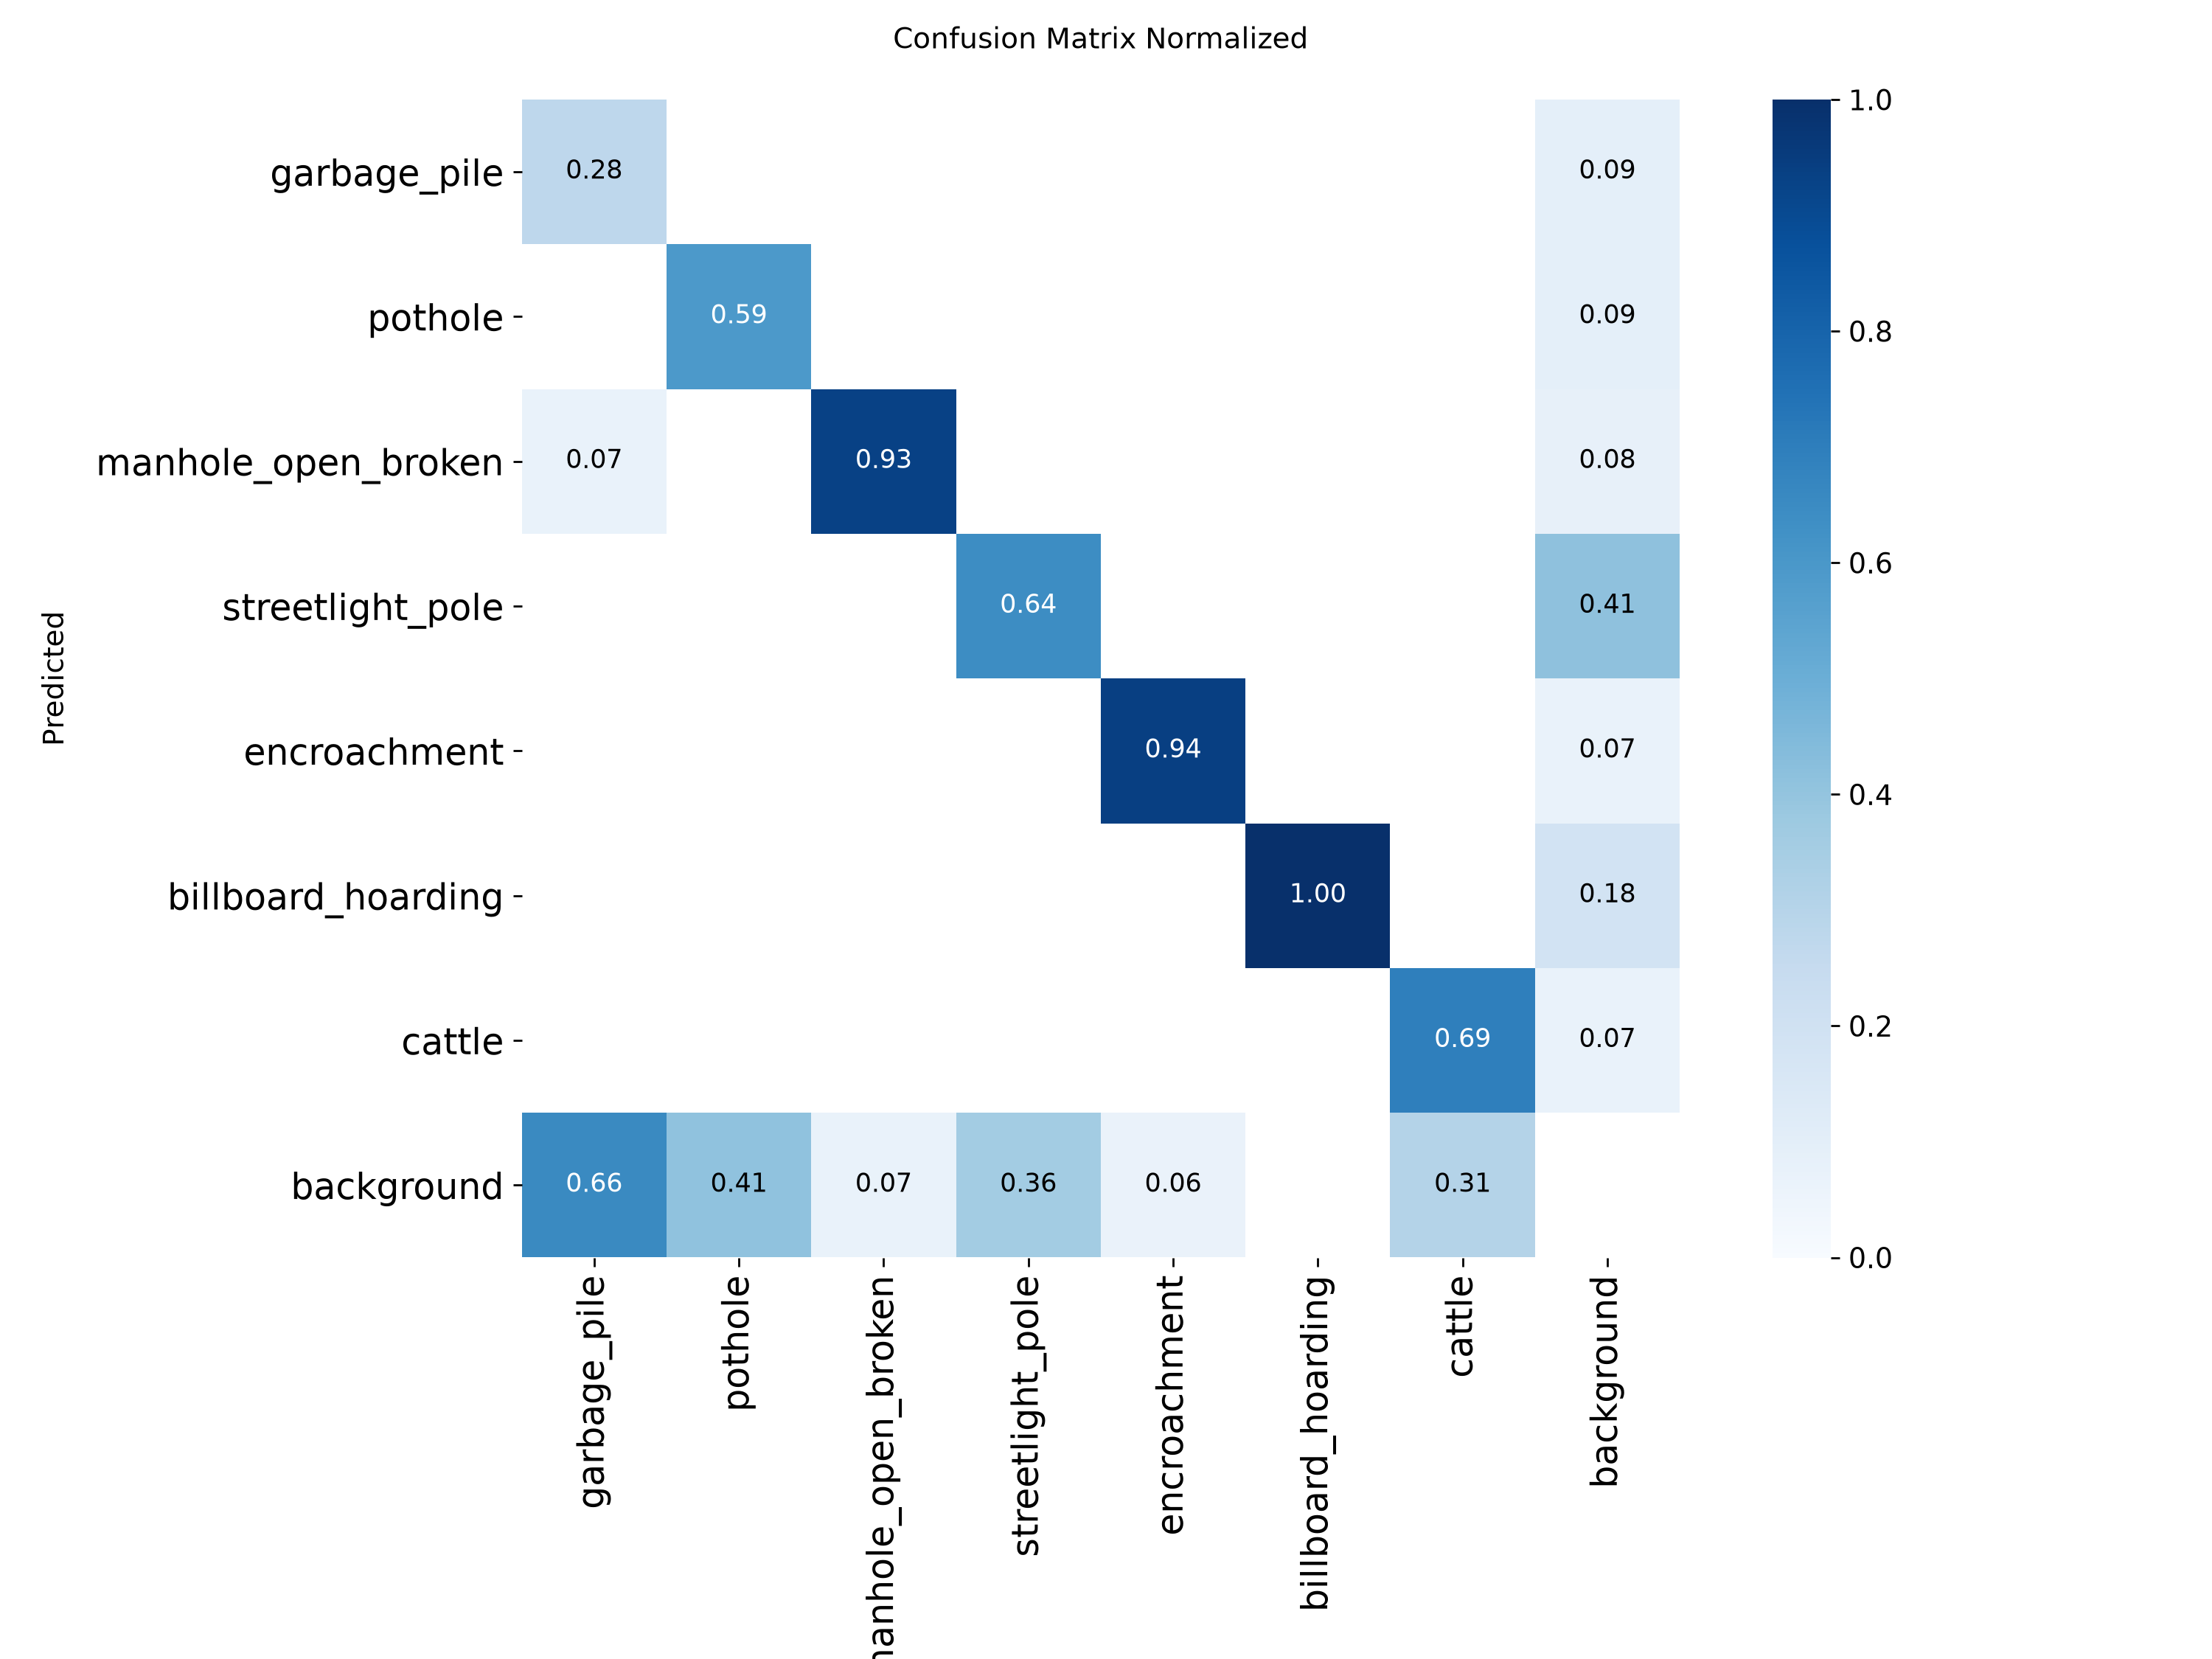
\includegraphics[width=\textwidth]{images/unbalanced_confusion_matrix_normalized.png}
    \caption{unbalanced}
  \end{subfigure}
  \hfill
  \begin{subfigure}{0.48\textwidth}
    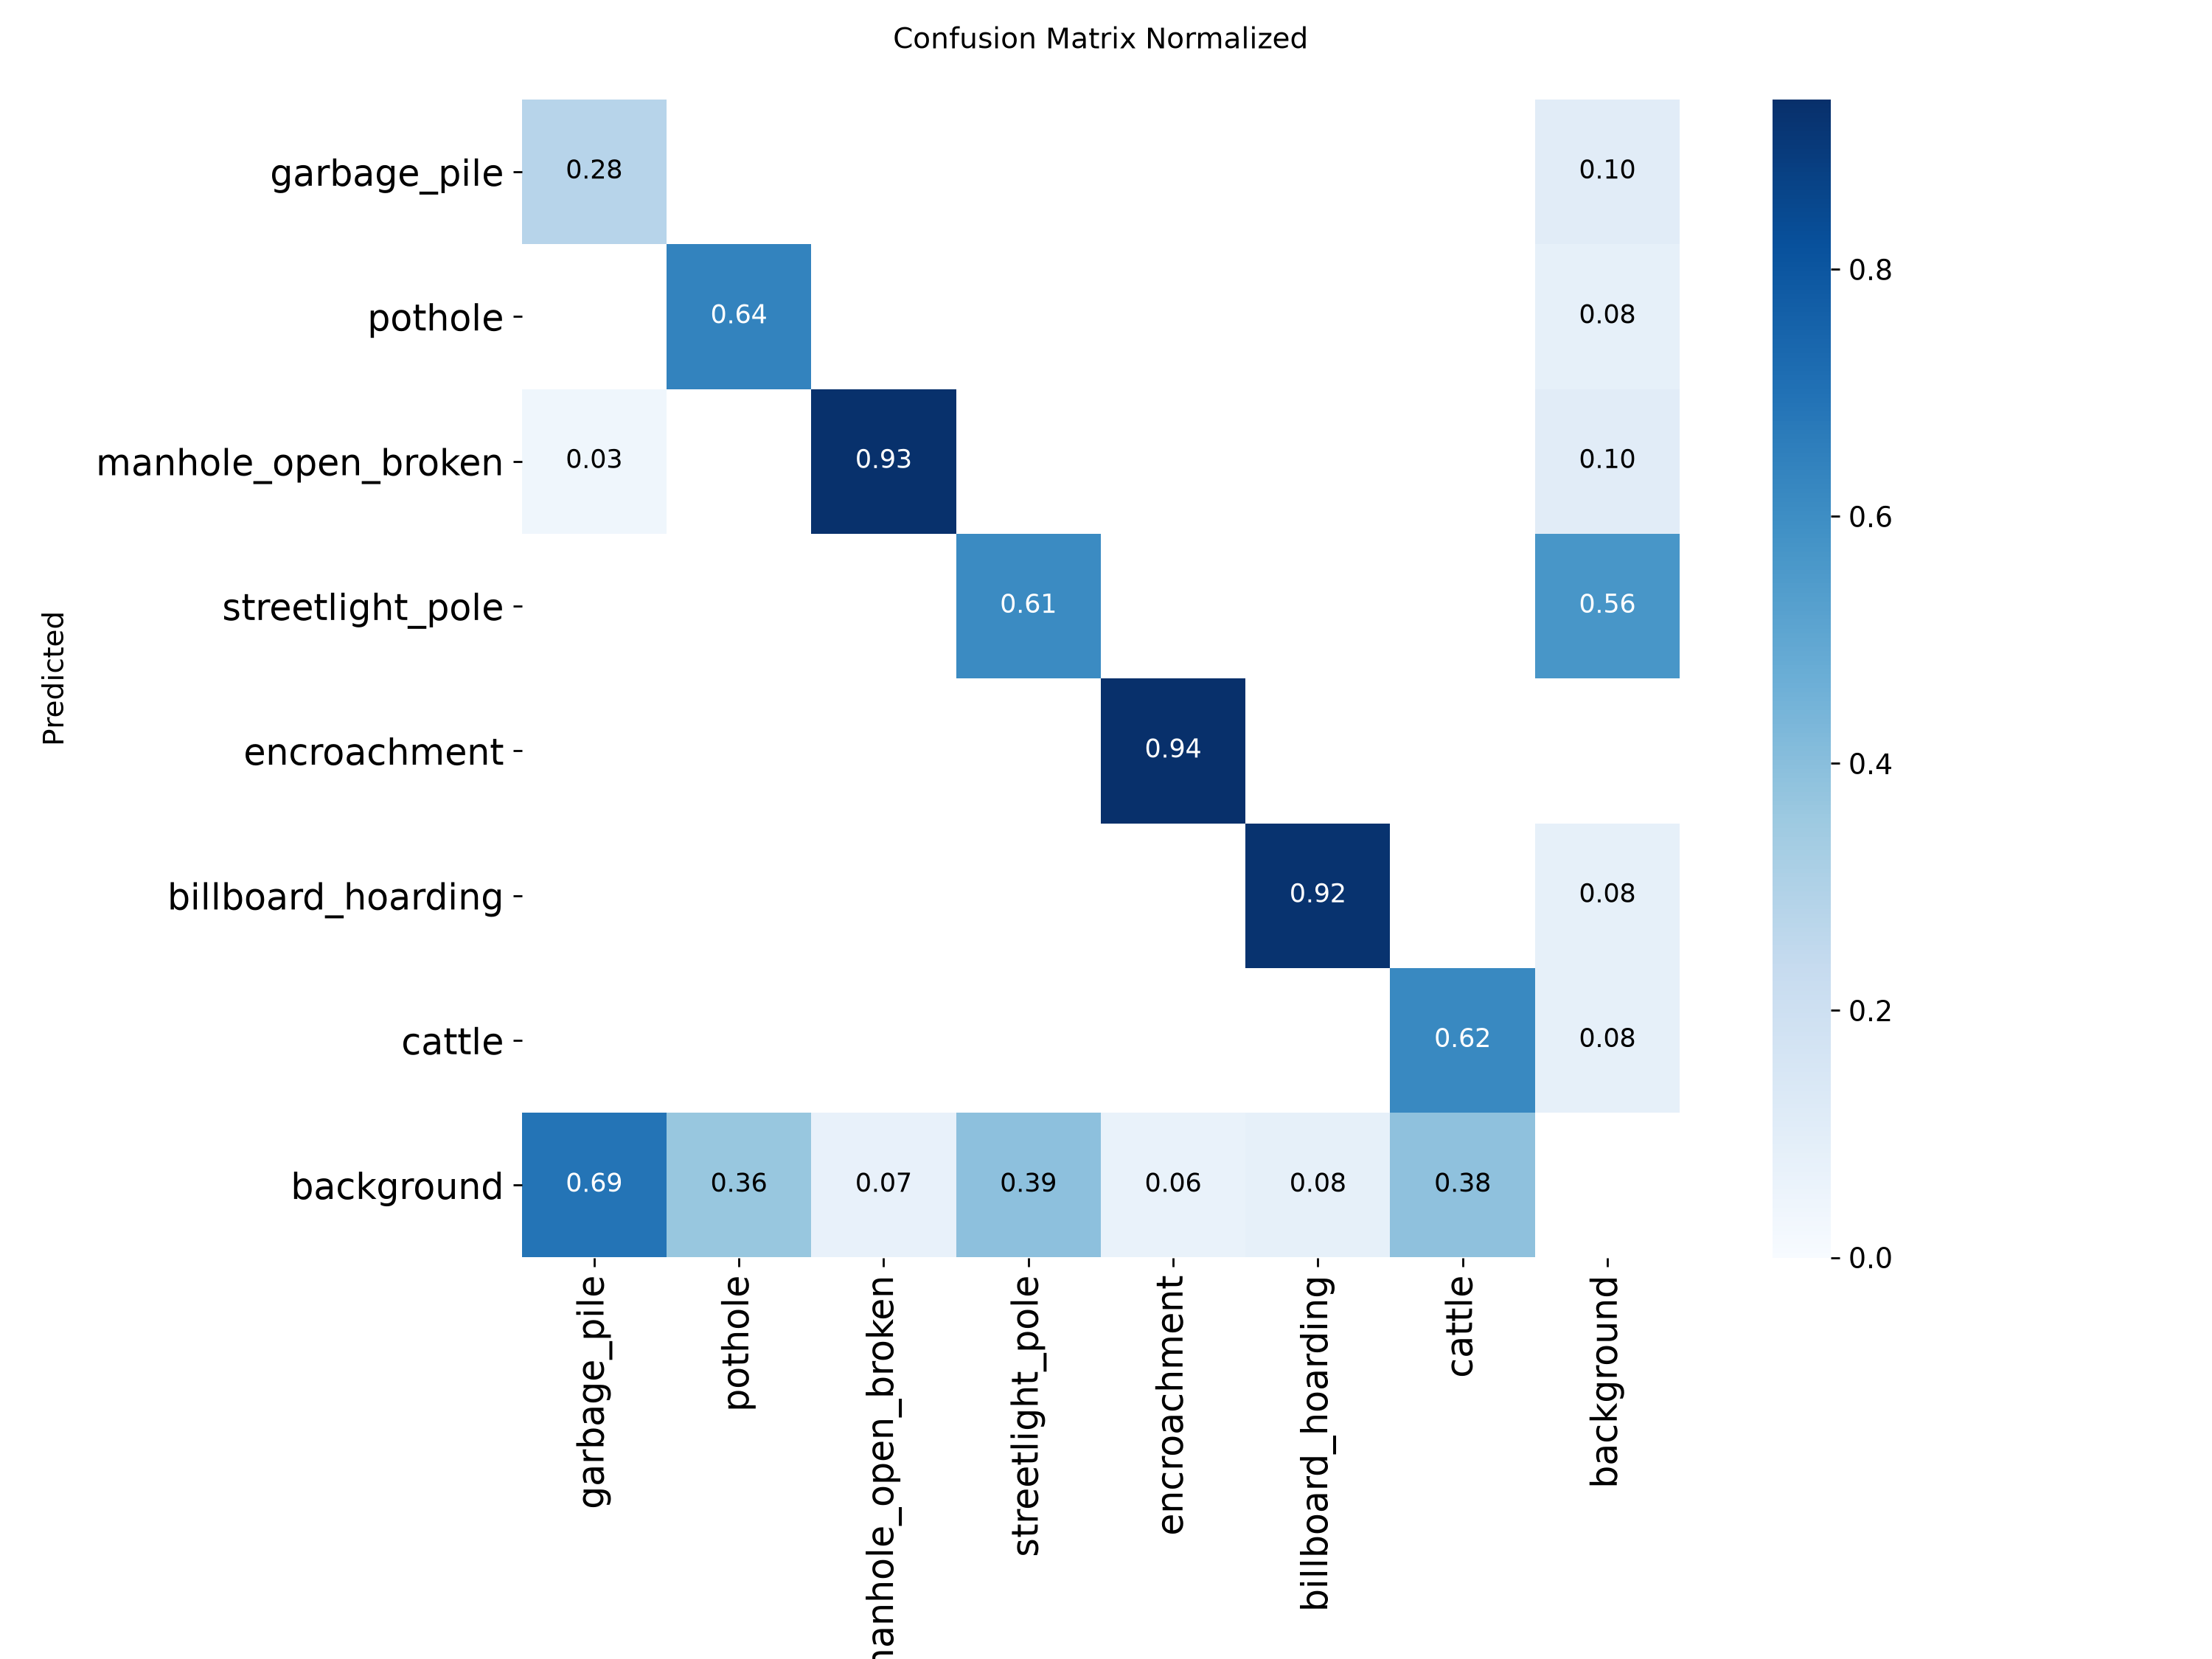
\includegraphics[width=\textwidth]{images/oversampled_confusion_matrix_normalized.png}
    \caption{oversampled}
  \end{subfigure}
  \caption{Normalized confusion matrices (rows = true class, background column captures
  missed/false detections). \texttt{garbage\_pile}'s weak diagonal in both matrices is the
  clearest visual confirmation of the AP50 weakness noted above.}
\end{figure}

\subsection{Precision-Recall Curves}

\begin{figure}[H]
  \centering
  \begin{subfigure}{0.48\textwidth}
    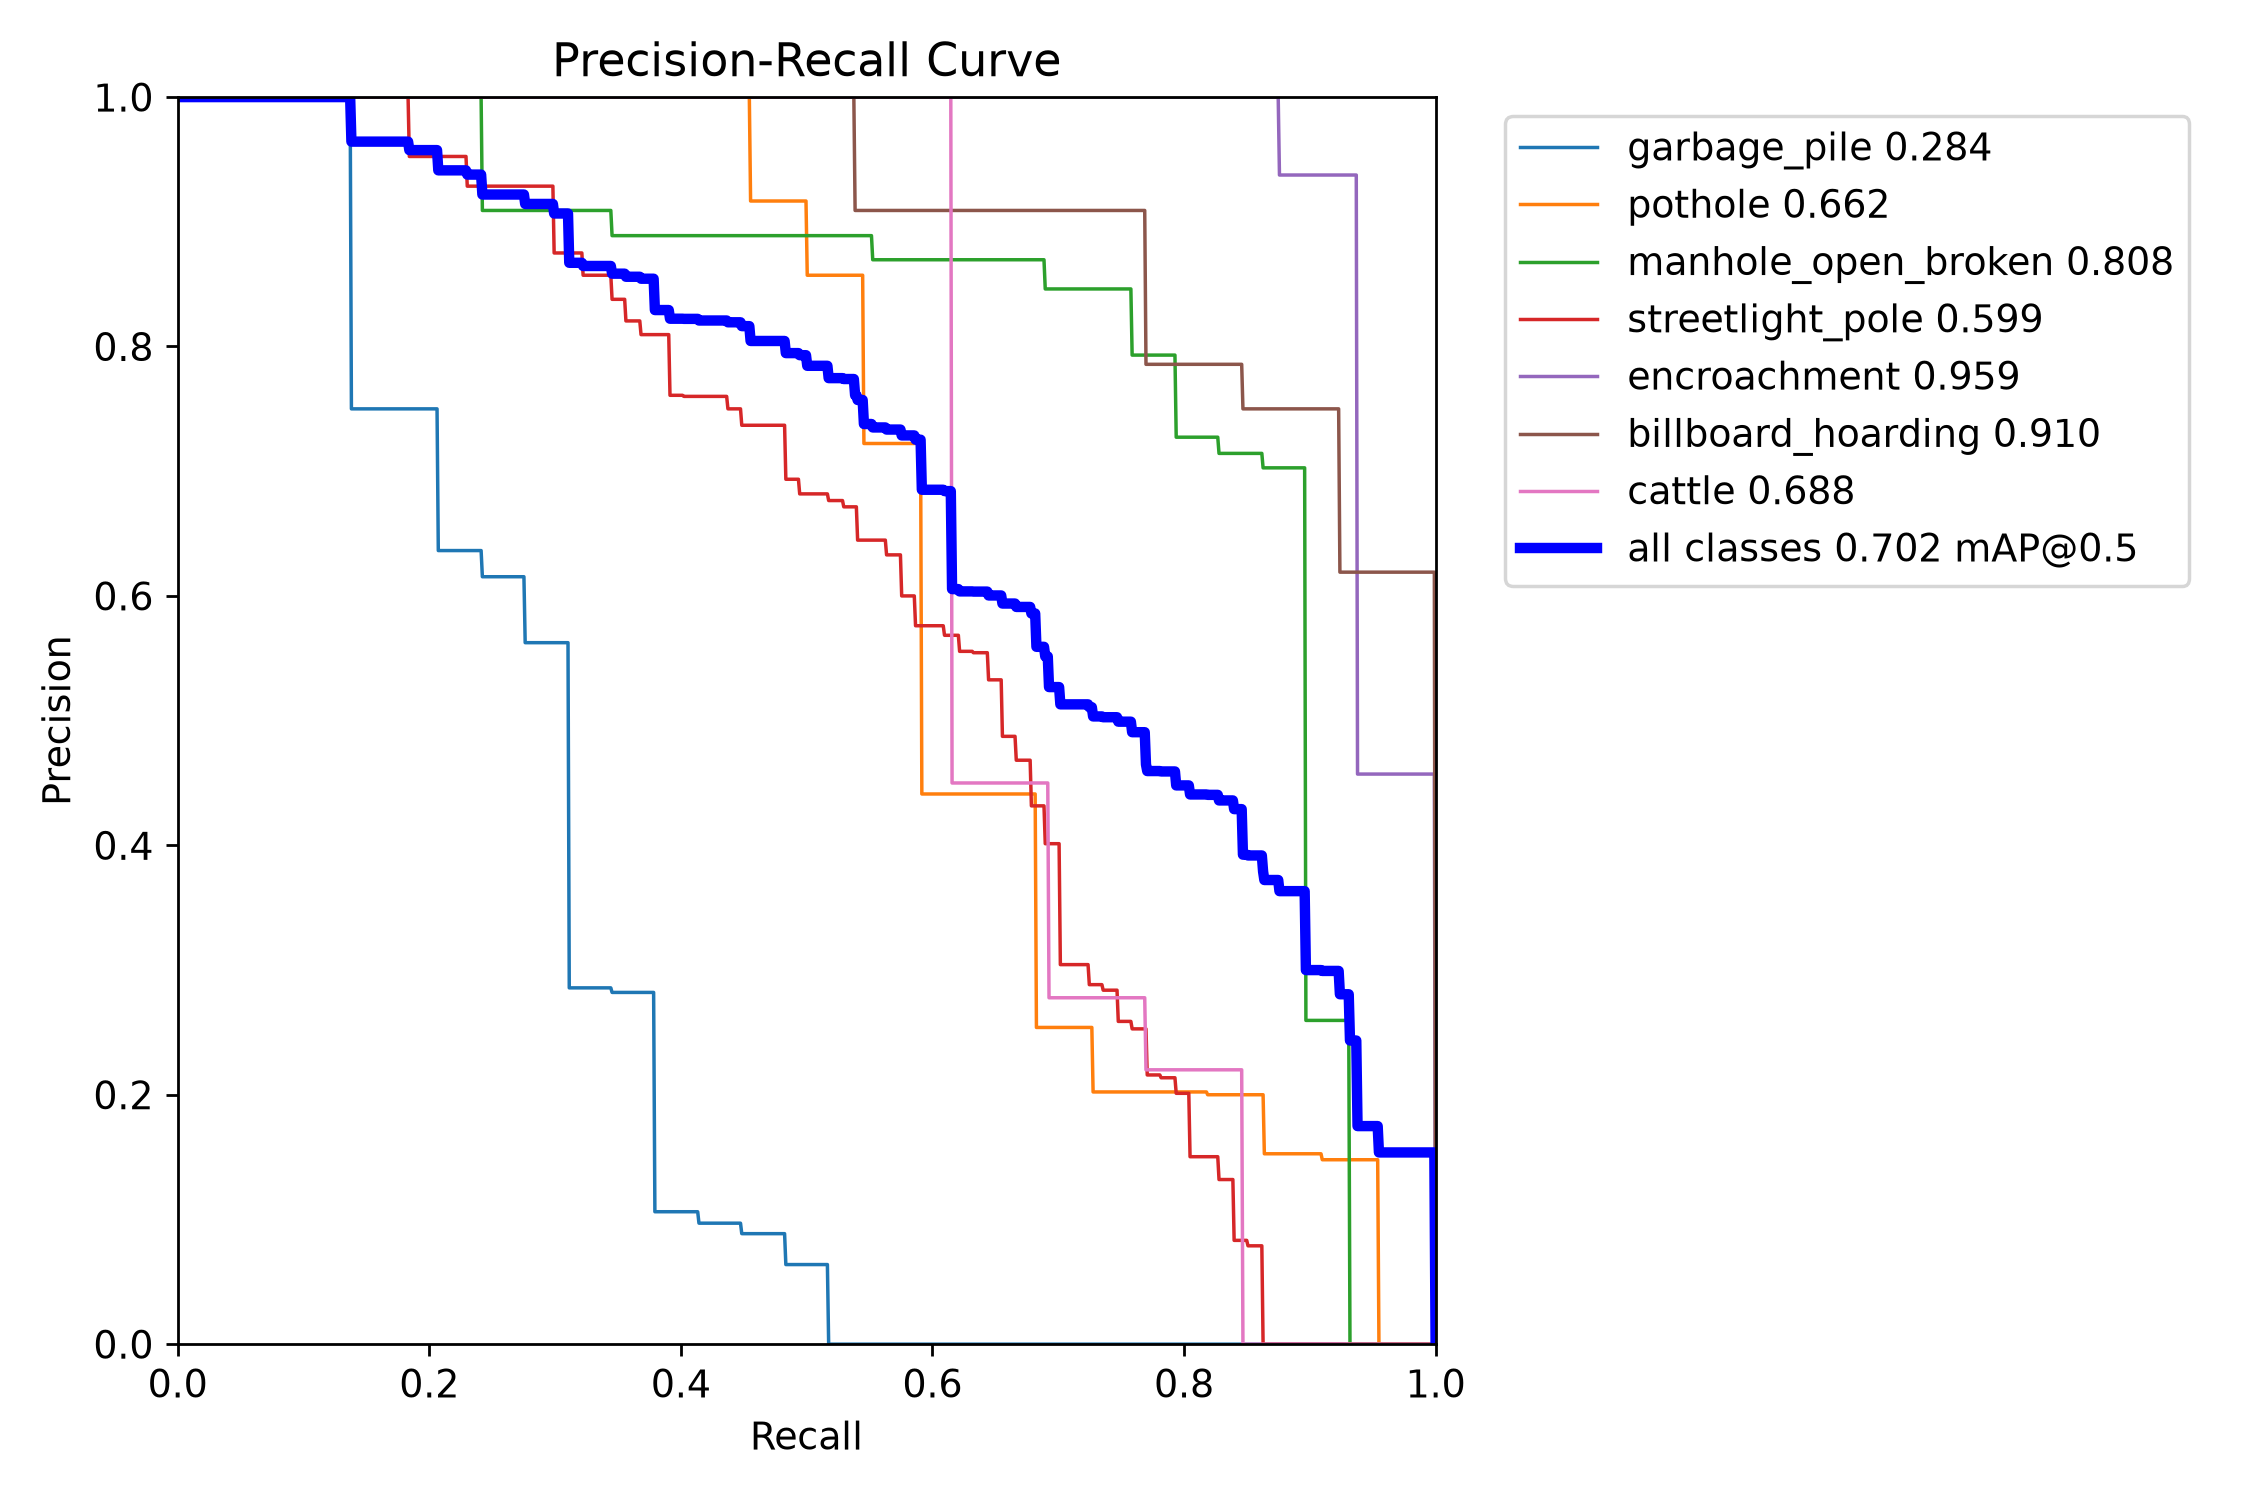
\includegraphics[width=\textwidth]{images/unbalanced_pr_curve.png}
    \caption{unbalanced}
  \end{subfigure}
  \hfill
  \begin{subfigure}{0.48\textwidth}
    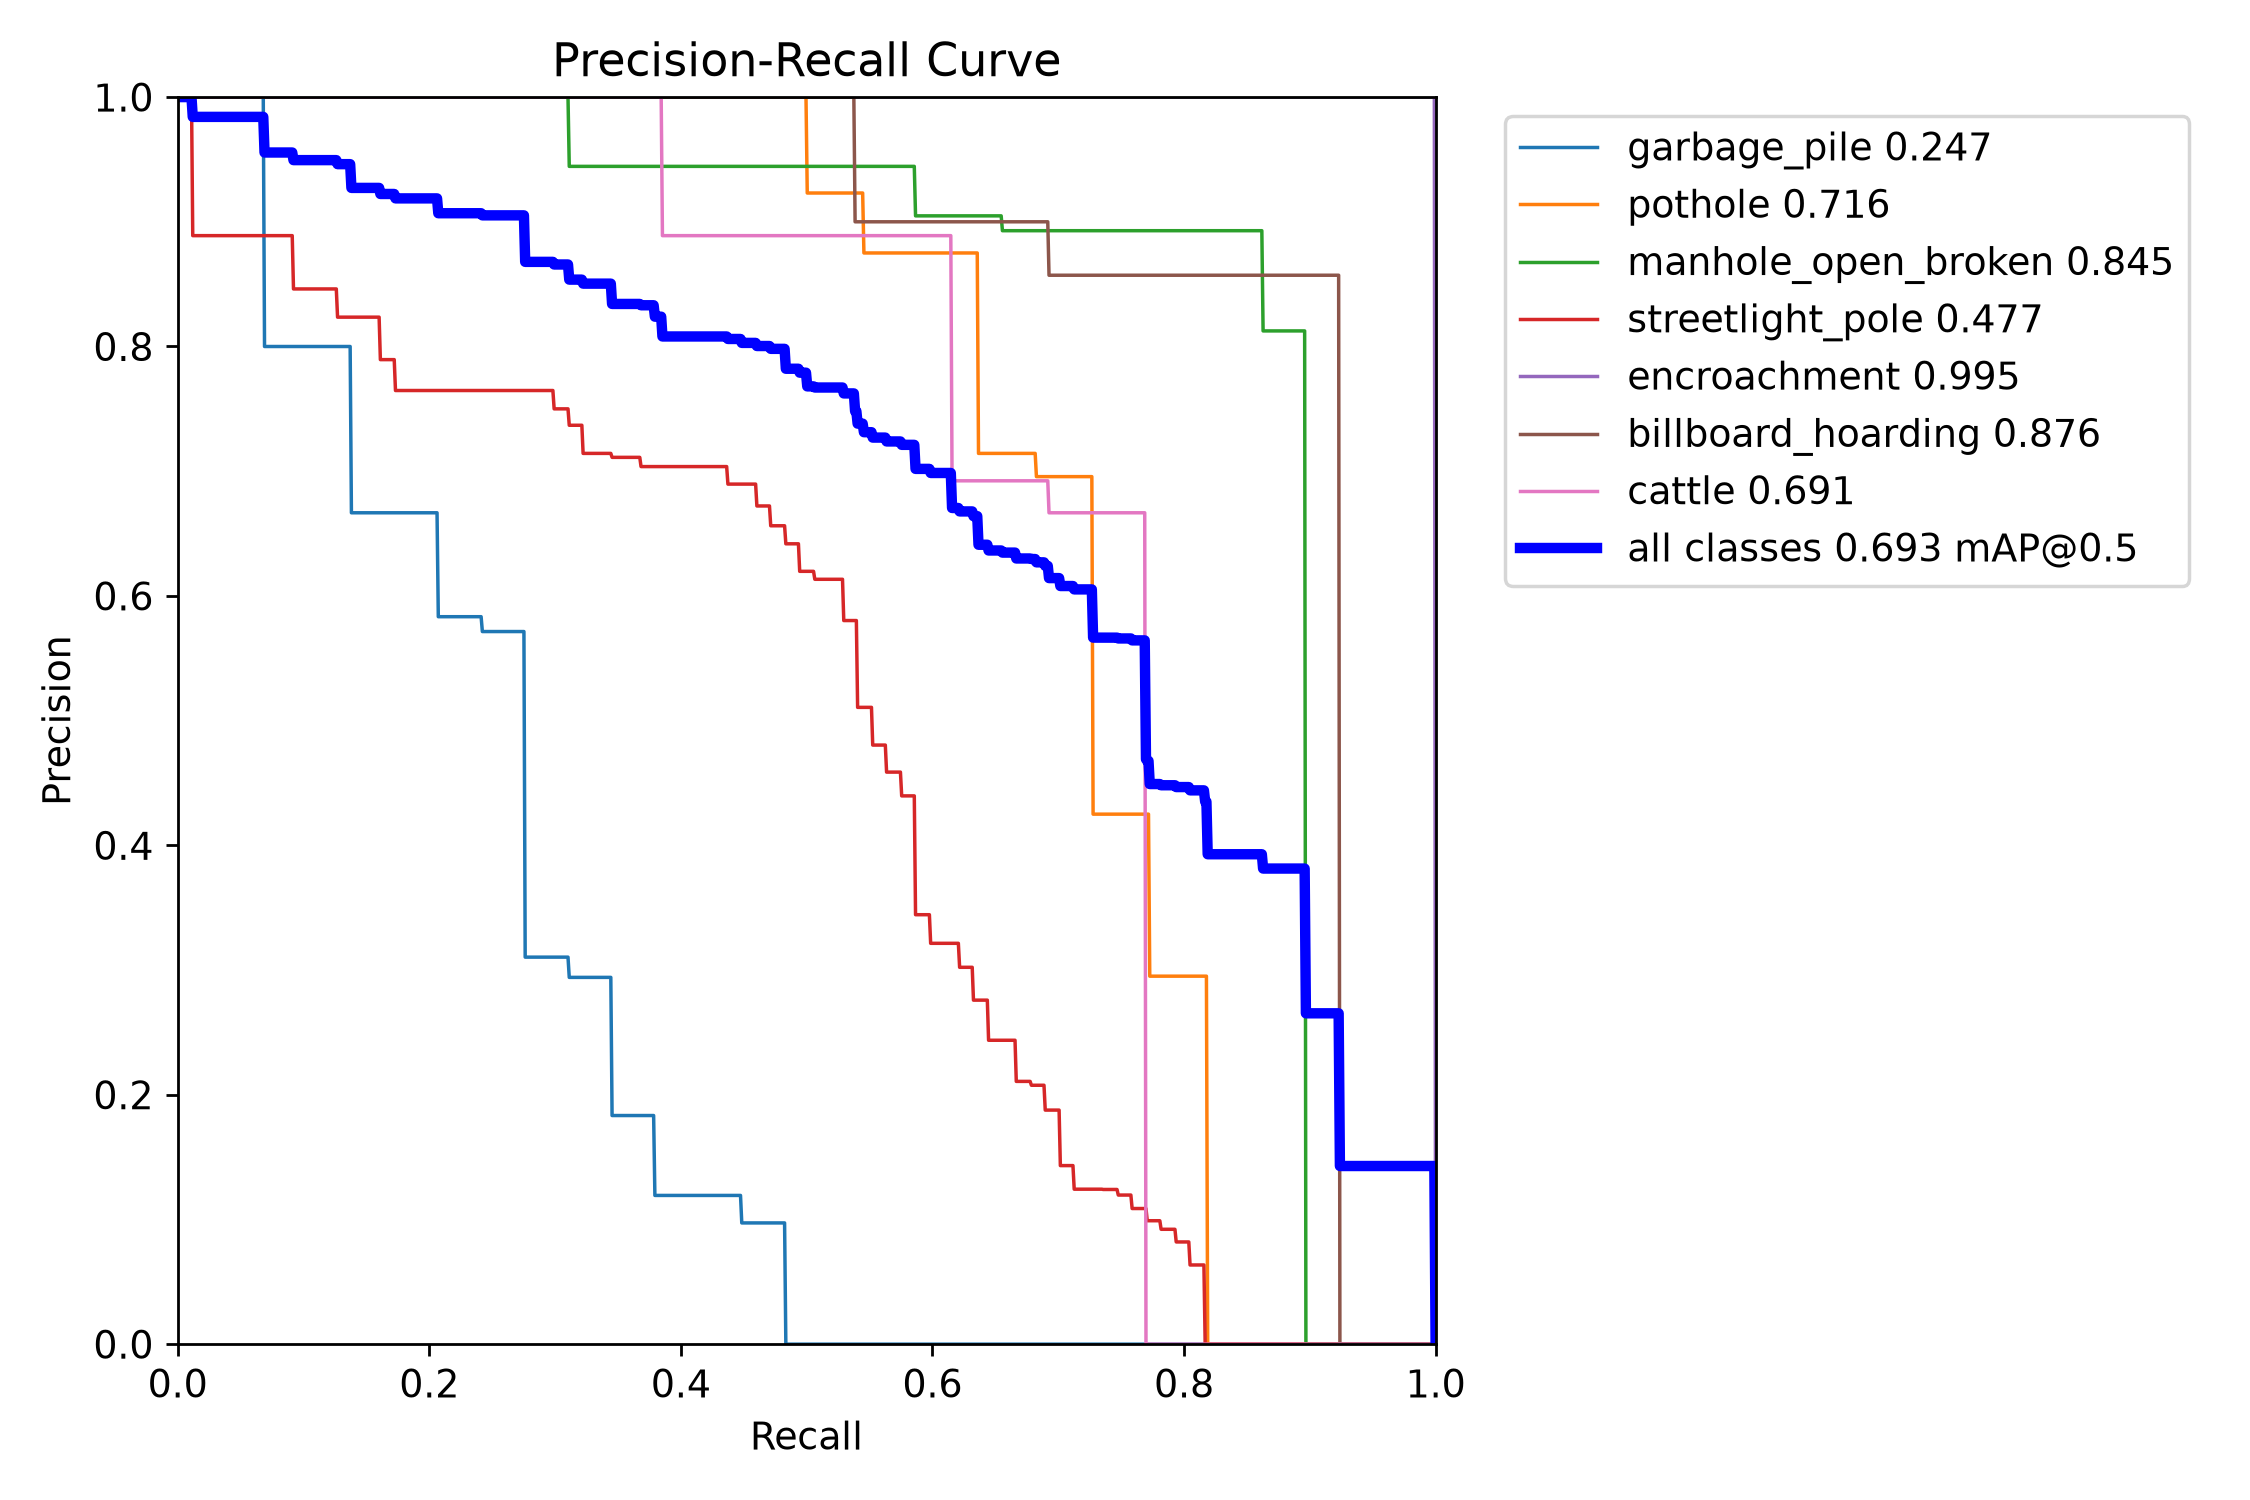
\includegraphics[width=\textwidth]{images/oversampled_pr_curve.png}
    \caption{oversampled}
  \end{subfigure}
  \caption{Per-class precision-recall curves. Note \texttt{streetlight\_pole}'s
  (orange/relevant curve) visibly lower area under oversampling, consistent with its
  AP50 regression.}
\end{figure}

% =====================================================================
\section{Overfitting Analysis}
% =====================================================================
Both runs show the classic overfitting signature: \textbf{training loss keeps falling for
all 100 epochs while validation loss plateaus around epoch 60--80 and barely moves after
that} — the train/val gap widens continuously instead of both curves flattening together.

\begin{table}[H]
\centering
\caption{Box-loss trend, selected epochs. Oversampled shows a larger absolute gap because
duplicated train images let the model partially memorize repeats.}
\begin{tabular}{lcccc}
\toprule
\textbf{Run} & \textbf{epoch} & \textbf{train\_box\_loss} & \textbf{val\_box\_loss} & \textbf{gap} \\
\midrule
unbalanced  & 40  & 1.291 & 1.838 & 0.547 \\
unbalanced  & 100 & 0.922 & 1.764 & \textbf{0.842} \\
\addlinespace
oversampled & 40  & 1.025 & 1.731 & 0.706 \\
oversampled & 100 & 0.642 & 1.689 & \textbf{1.047} \\
\bottomrule
\end{tabular}
\end{table}

mAP50-95 peaks around epoch 83--85 in both runs and only wobbles afterward — the extra
$\sim$15--20 epochs of training past that point are not buying further generalization.
\texttt{train.py}'s early-stopping \texttt{patience} is set to 20 and never triggered
(each 20-epoch window still produced a marginal new best), so tightening it (e.g.\ to 10)
would likely reach an equivalent result faster without changing outcomes, since
Ultralytics already saves \texttt{best.pt} at the true best epoch rather than the final one.

\begin{figure}[H]
  \centering
  \begin{subfigure}{0.48\textwidth}
    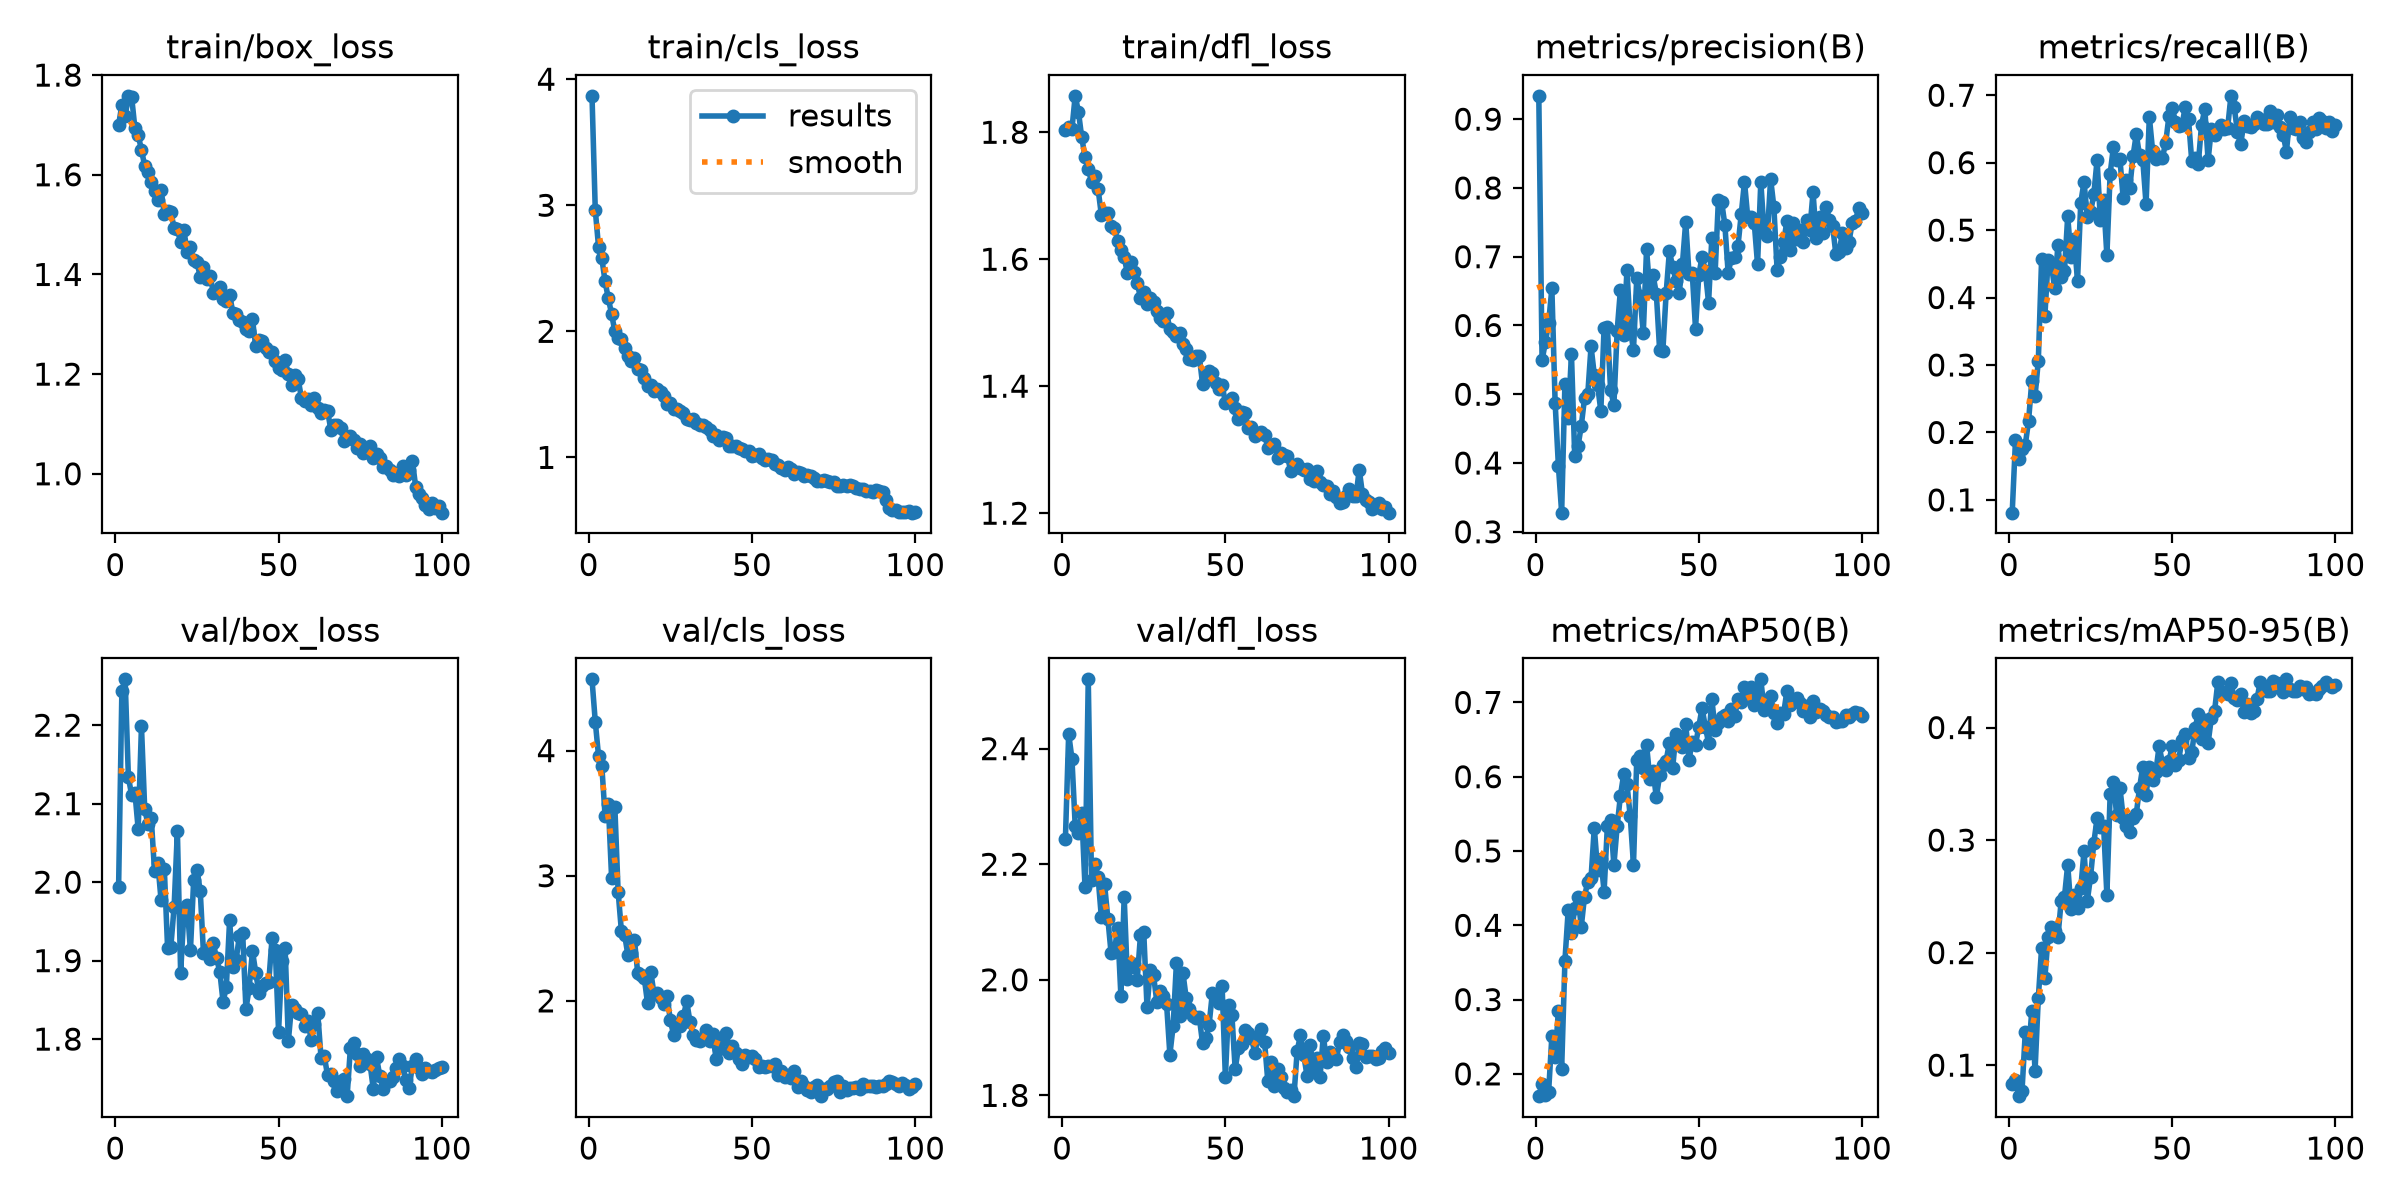
\includegraphics[width=\textwidth]{images/unbalanced_results.png}
    \caption{unbalanced}
  \end{subfigure}
  \hfill
  \begin{subfigure}{0.48\textwidth}
    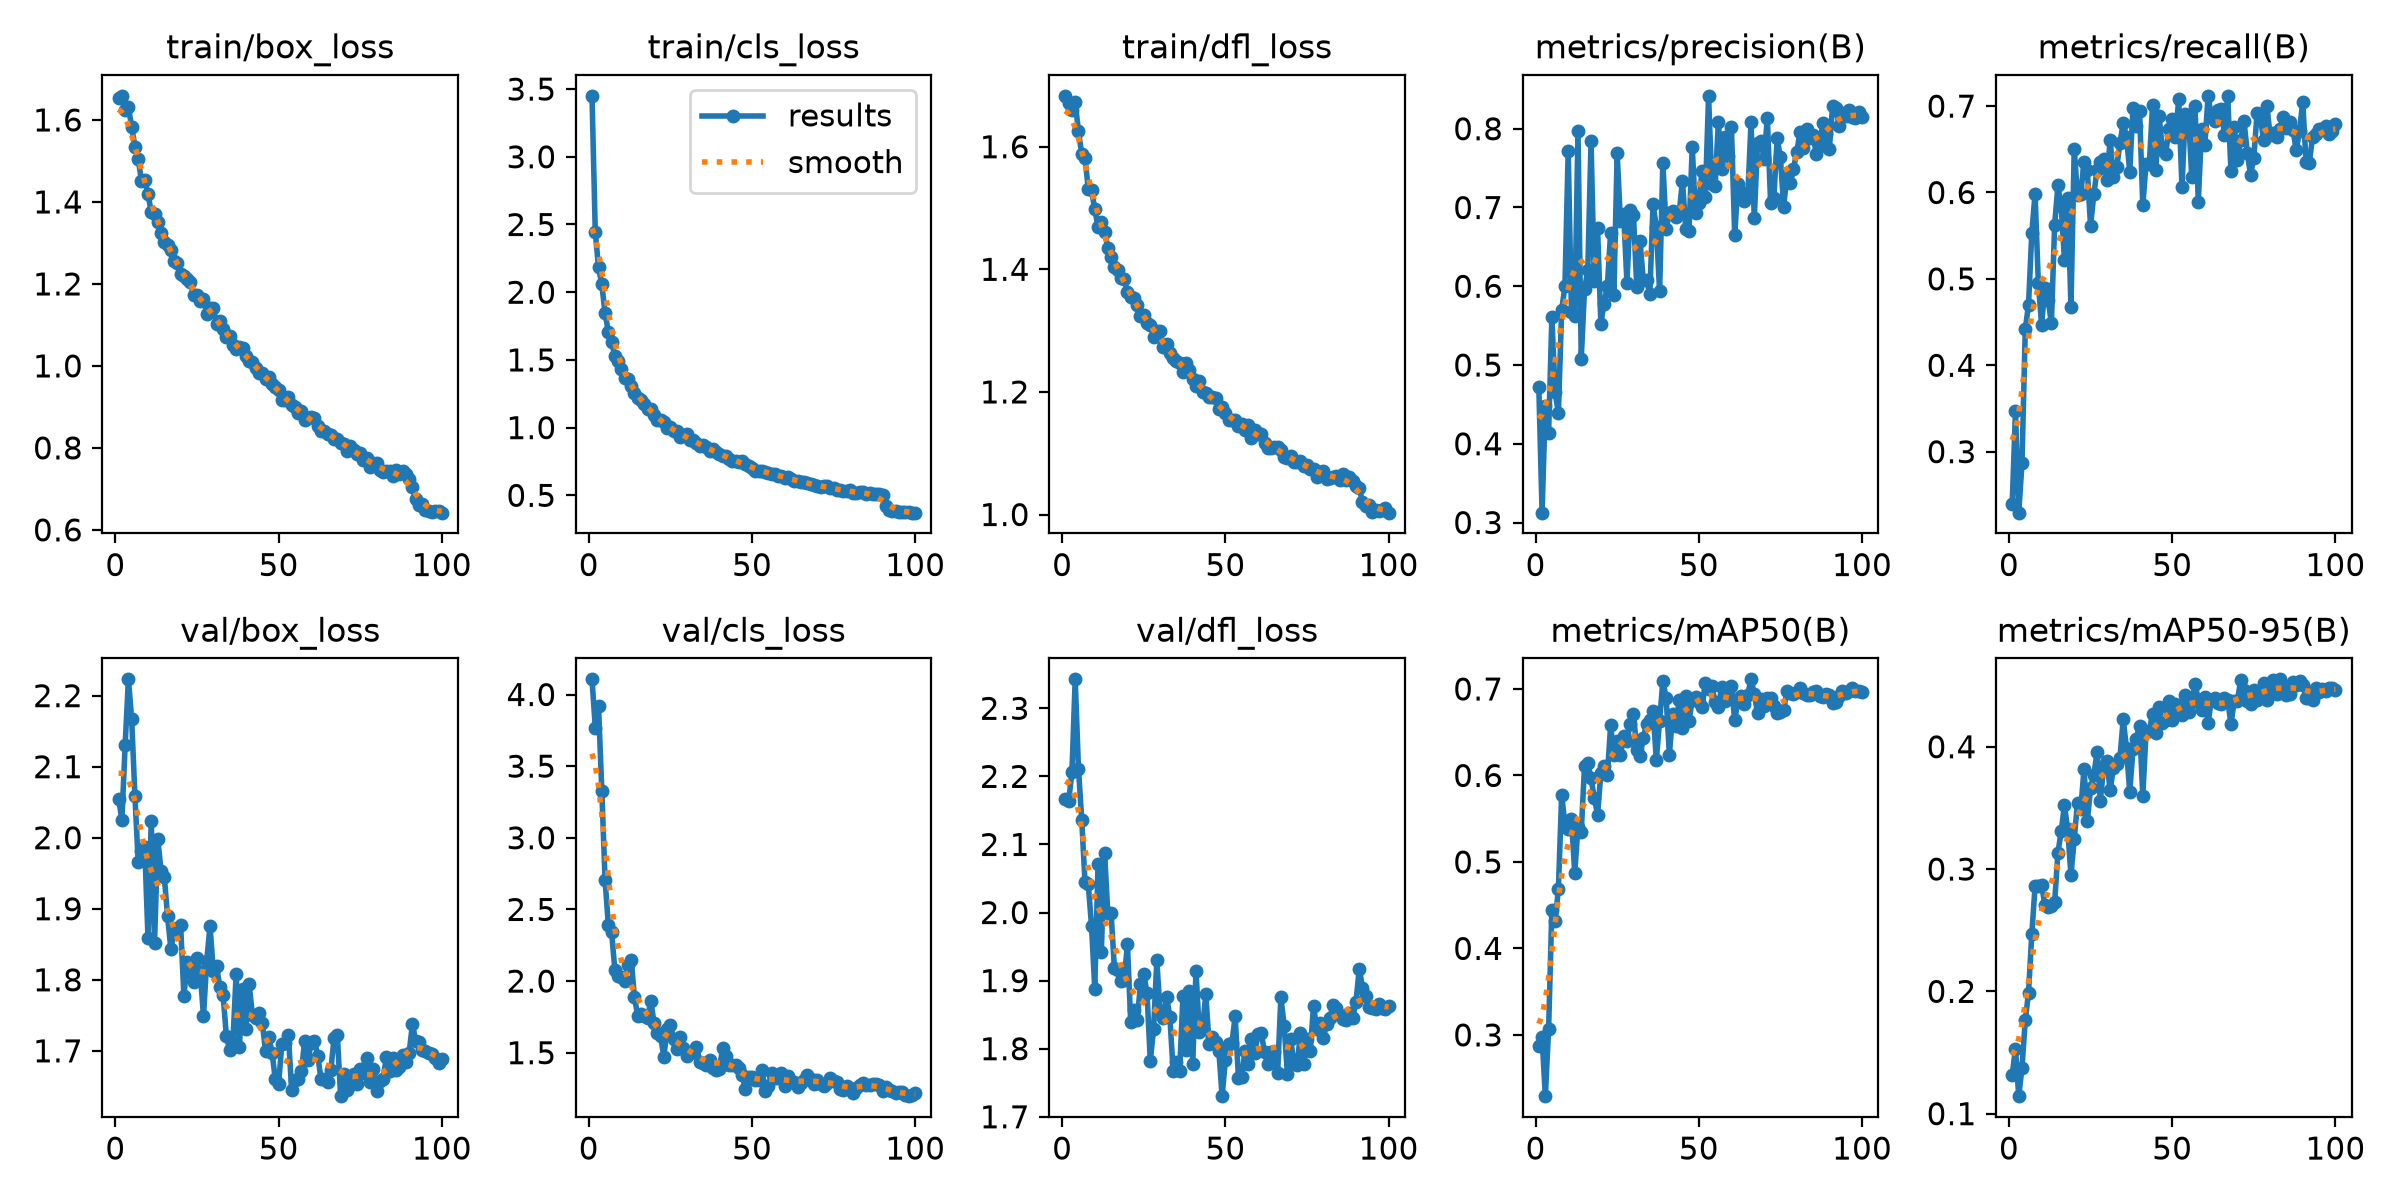
\includegraphics[width=\textwidth]{images/oversampled_results.png}
    \caption{oversampled}
  \end{subfigure}
  \caption{Full per-epoch loss/metric curves. In both, the box/cls/dfl loss panels show
  train (blue) diverging from val (orange) after roughly epoch 60--80.}
\end{figure}

% =====================================================================
\section{Qualitative Detection Samples}
% =====================================================================
\begin{figure}[H]
  \centering
  \begin{subfigure}{0.48\textwidth}
    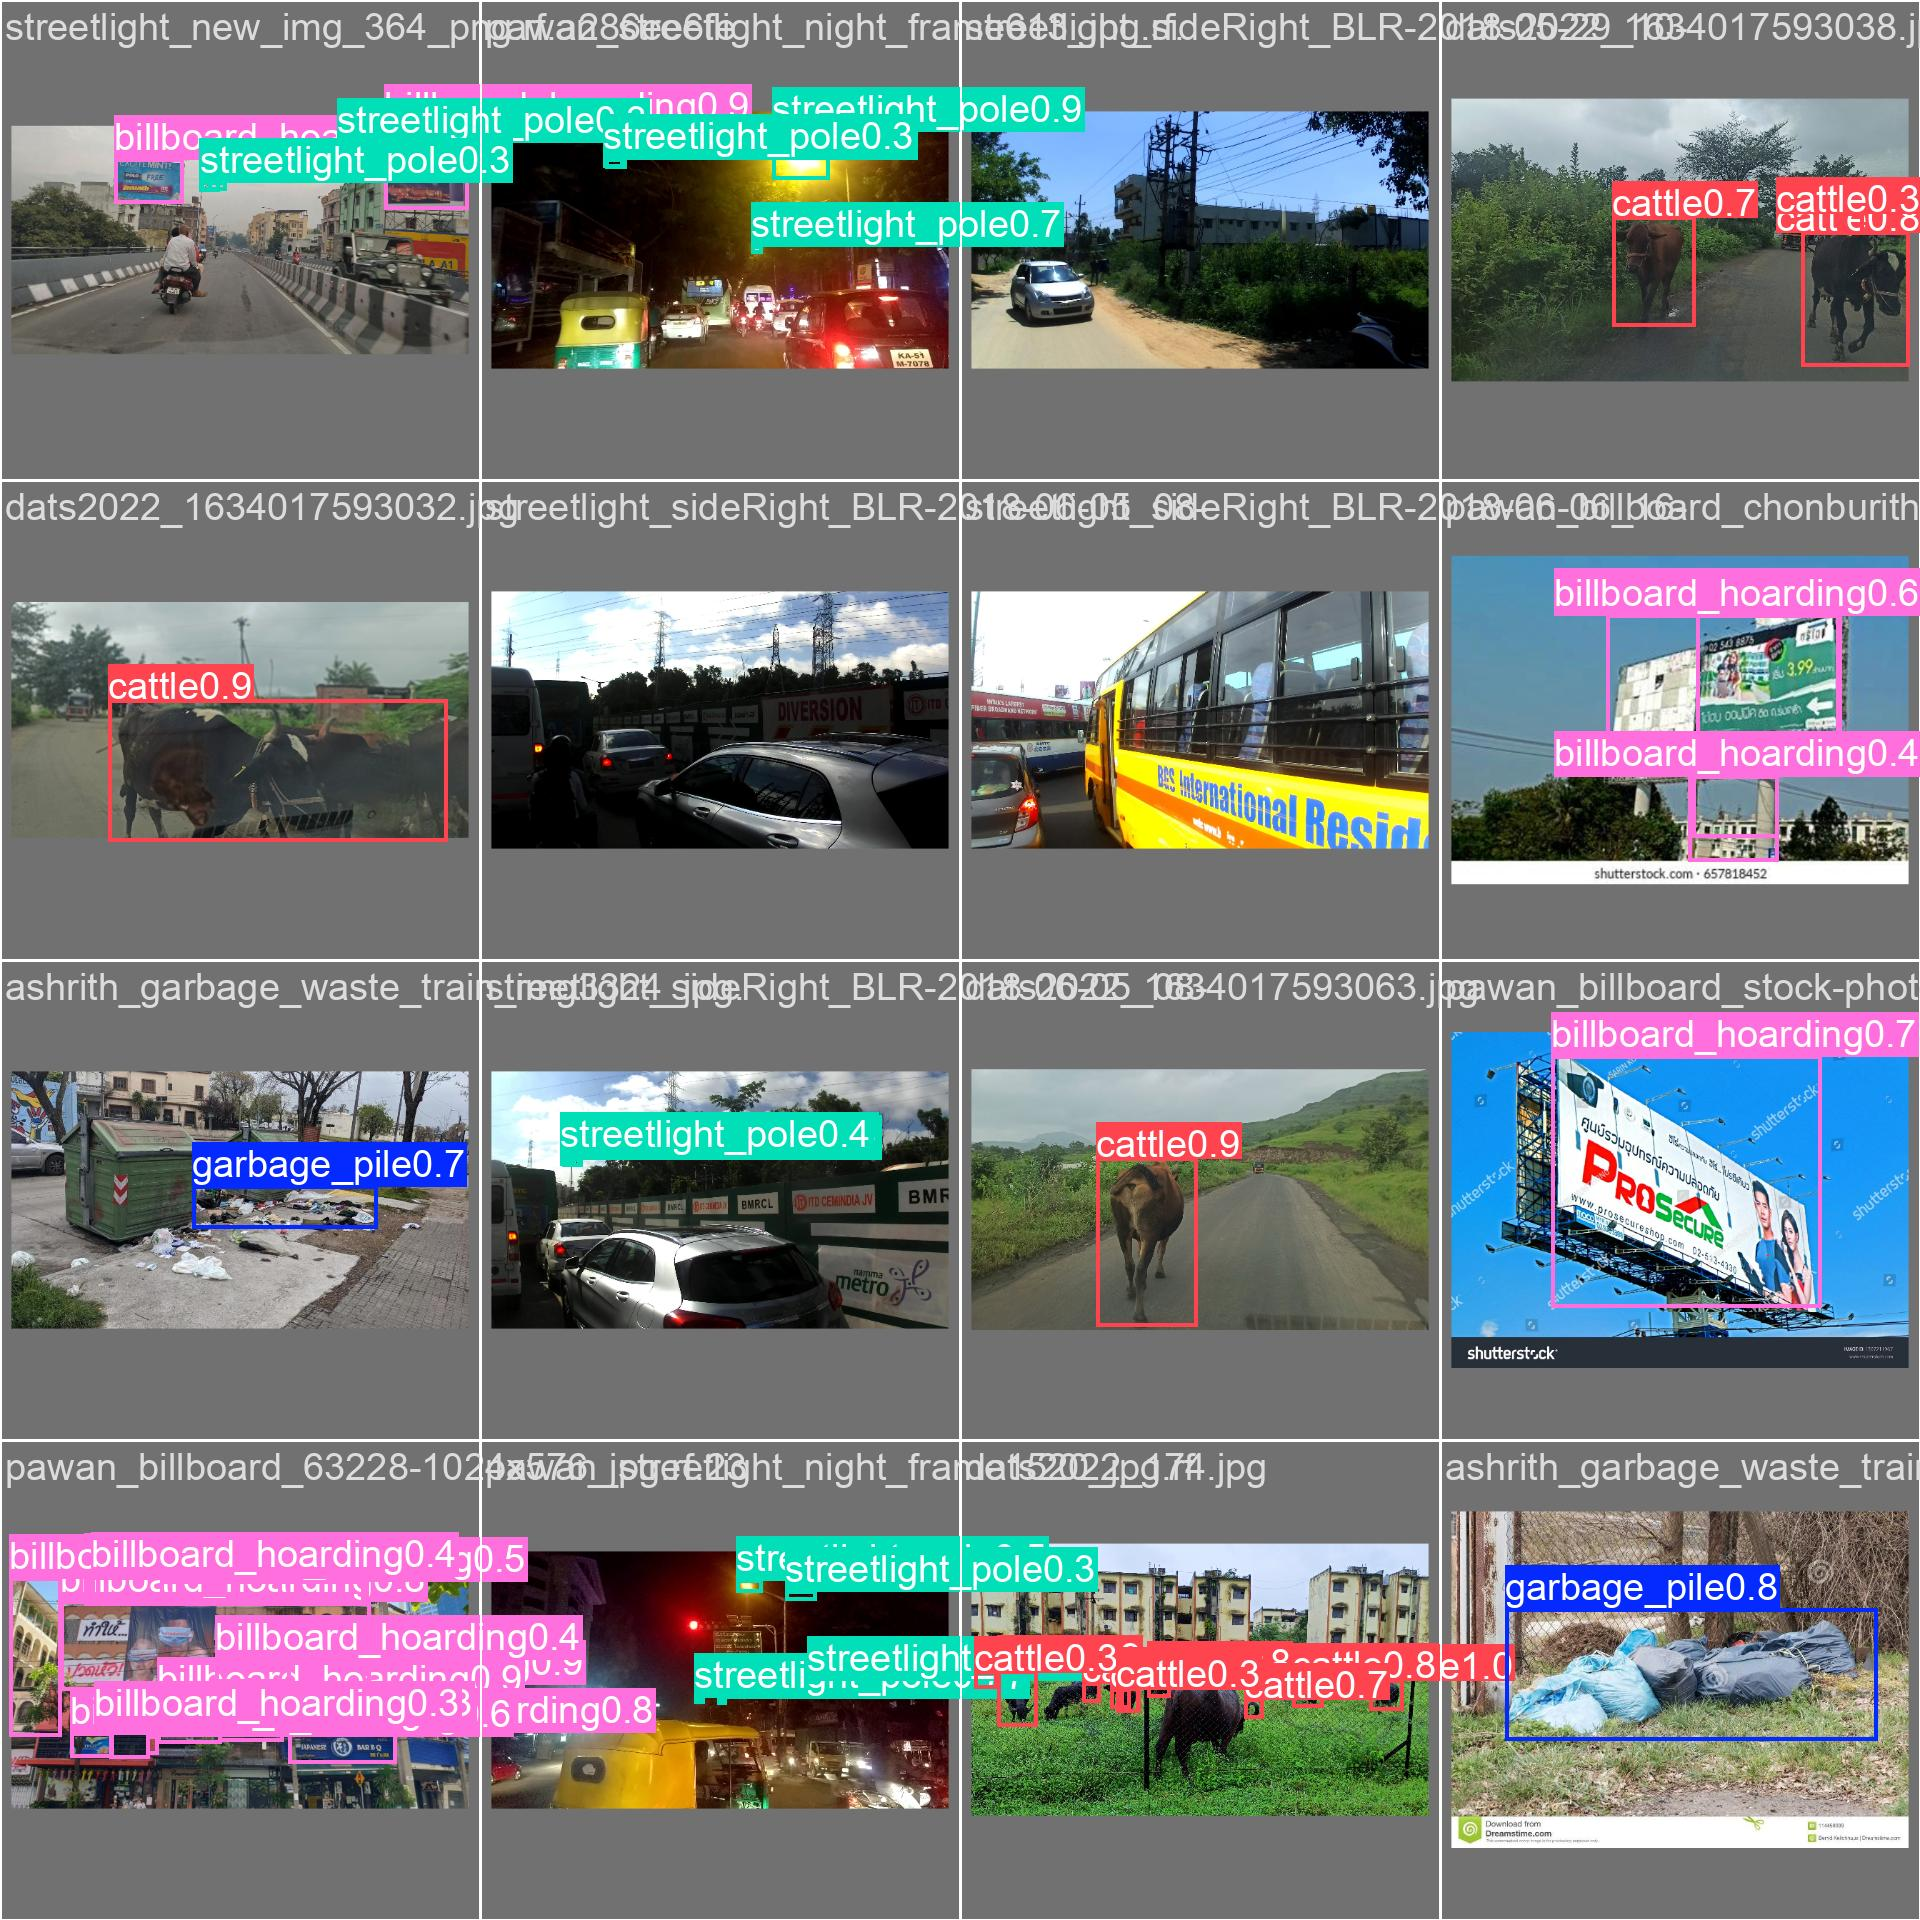
\includegraphics[width=\textwidth]{images/unbalanced_val_pred.jpg}
    \caption{unbalanced — val batch predictions}
  \end{subfigure}
  \hfill
  \begin{subfigure}{0.48\textwidth}
    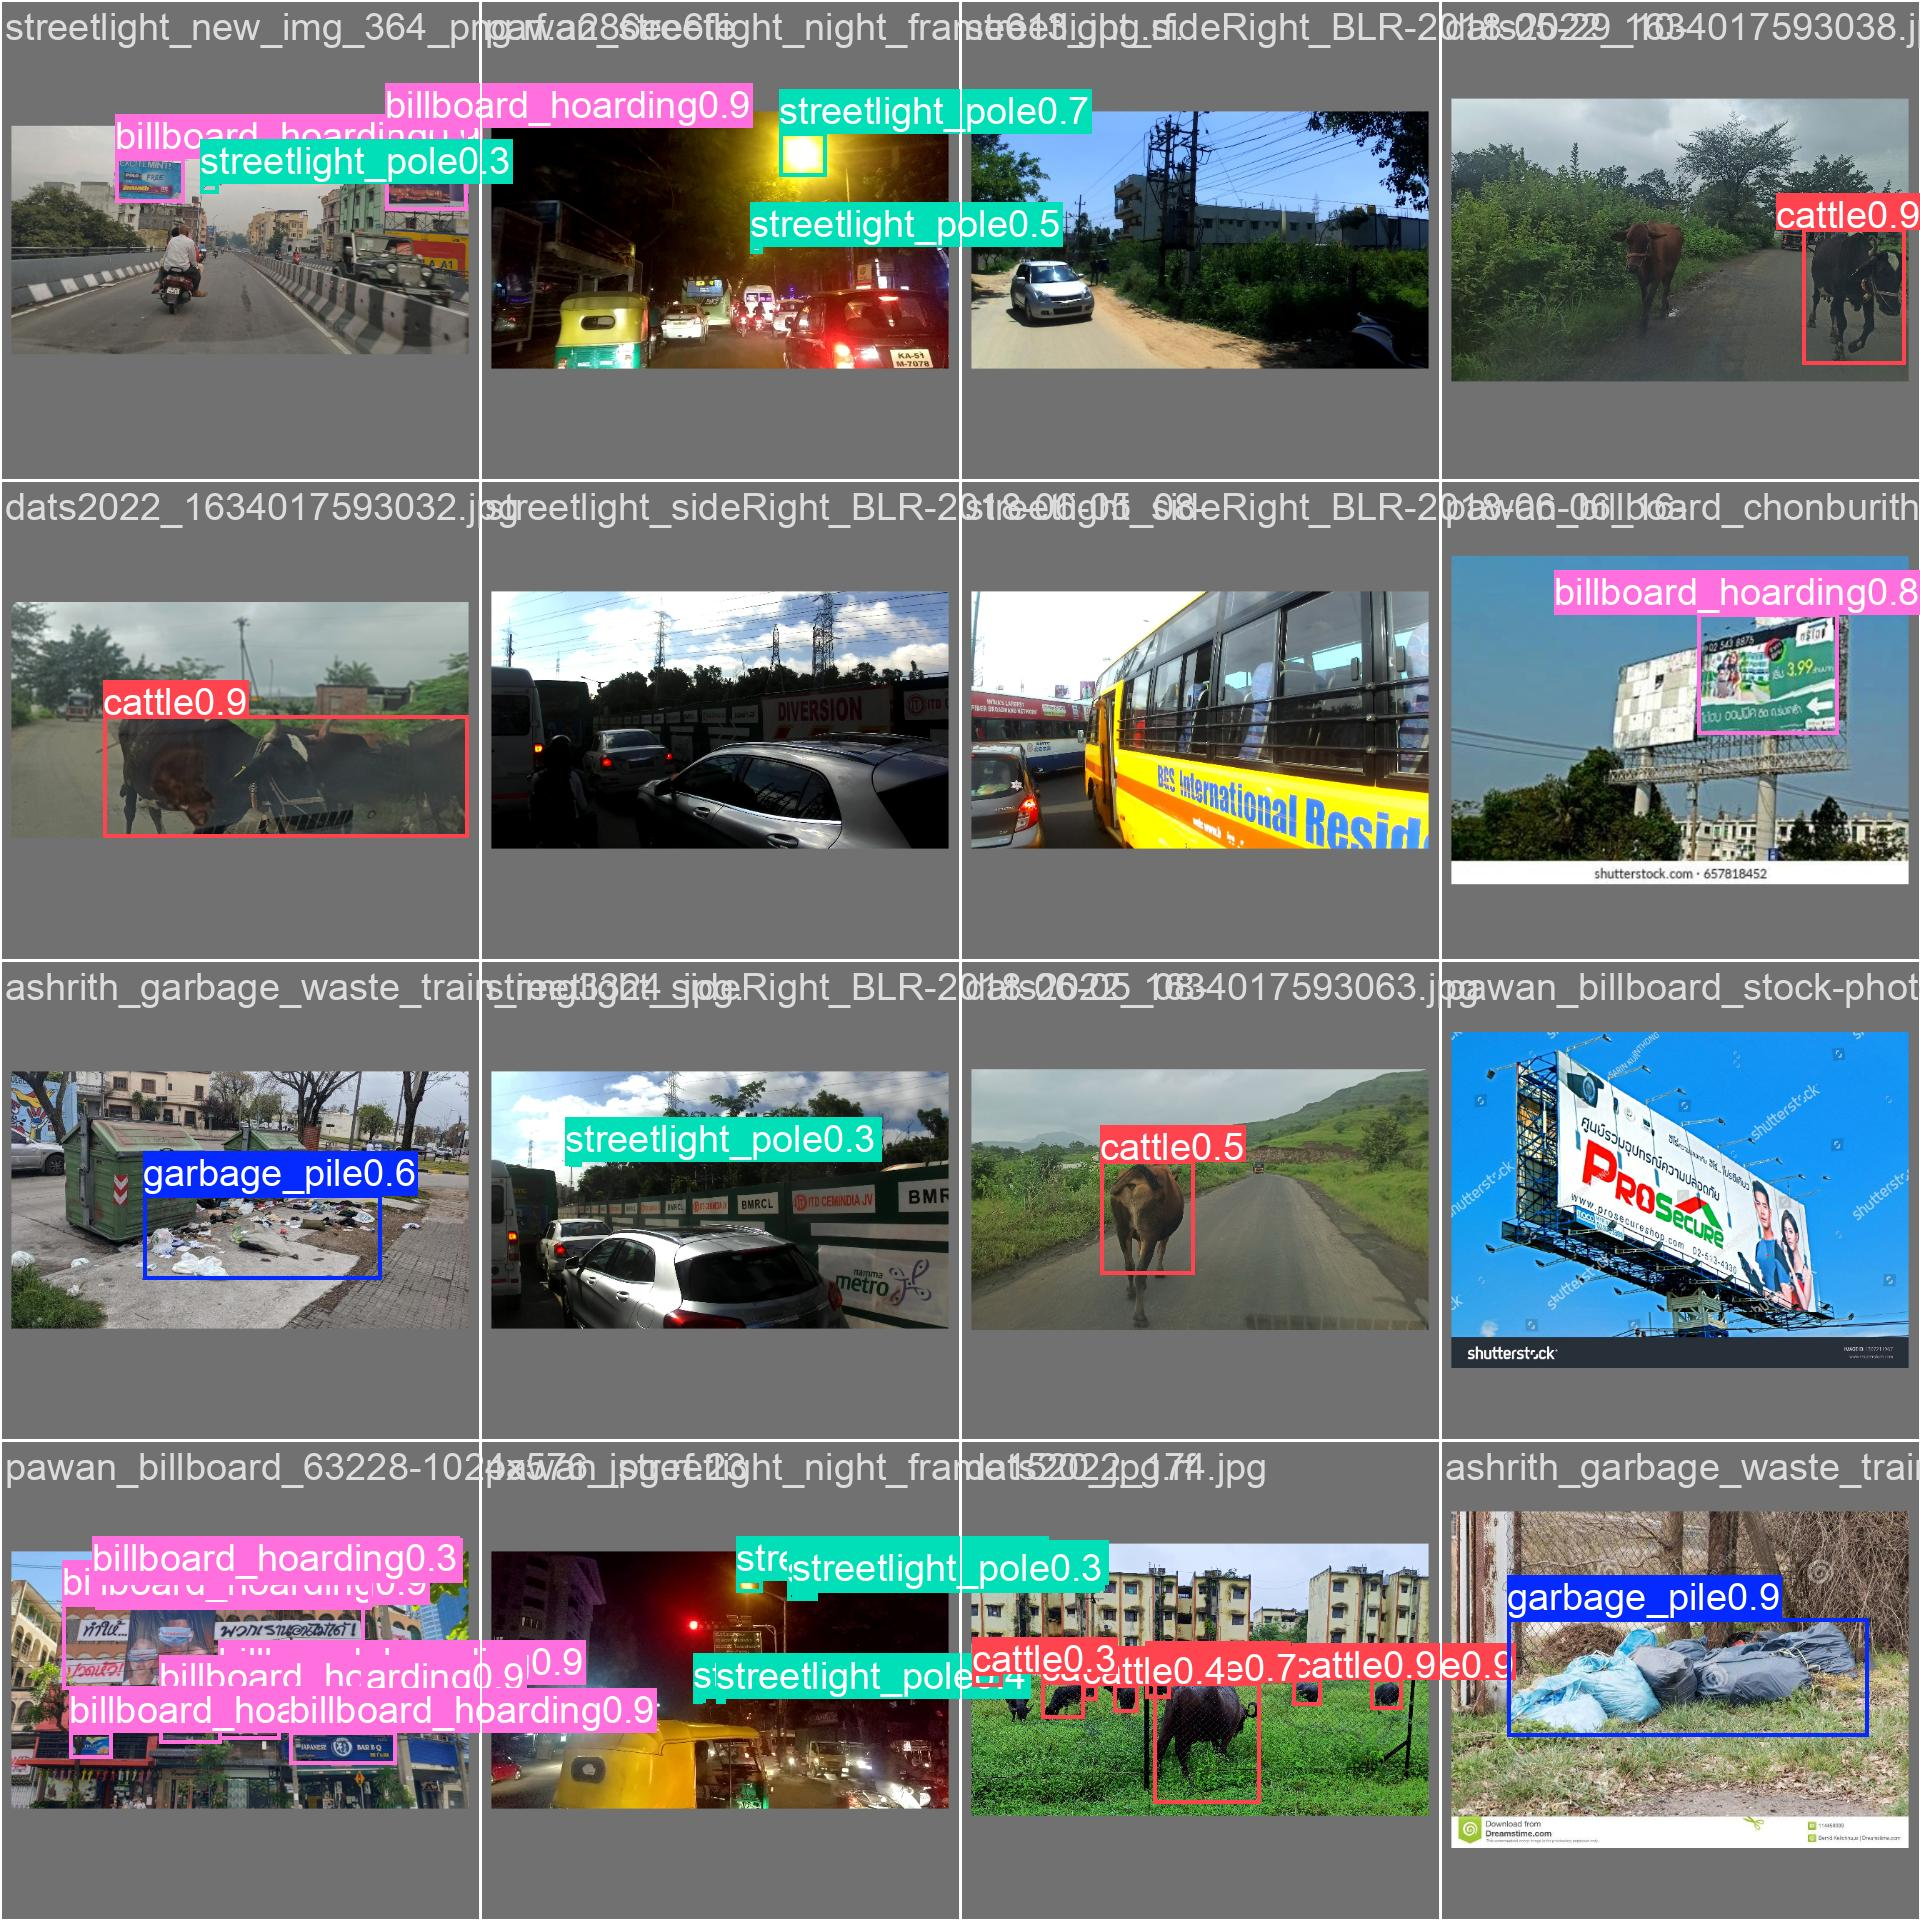
\includegraphics[width=\textwidth]{images/oversampled_val_pred.jpg}
    \caption{oversampled — val batch predictions}
  \end{subfigure}
  \caption{Model predictions on the same held-out validation batch for each run.}
\end{figure}

\begin{figure}[H]
  \centering
  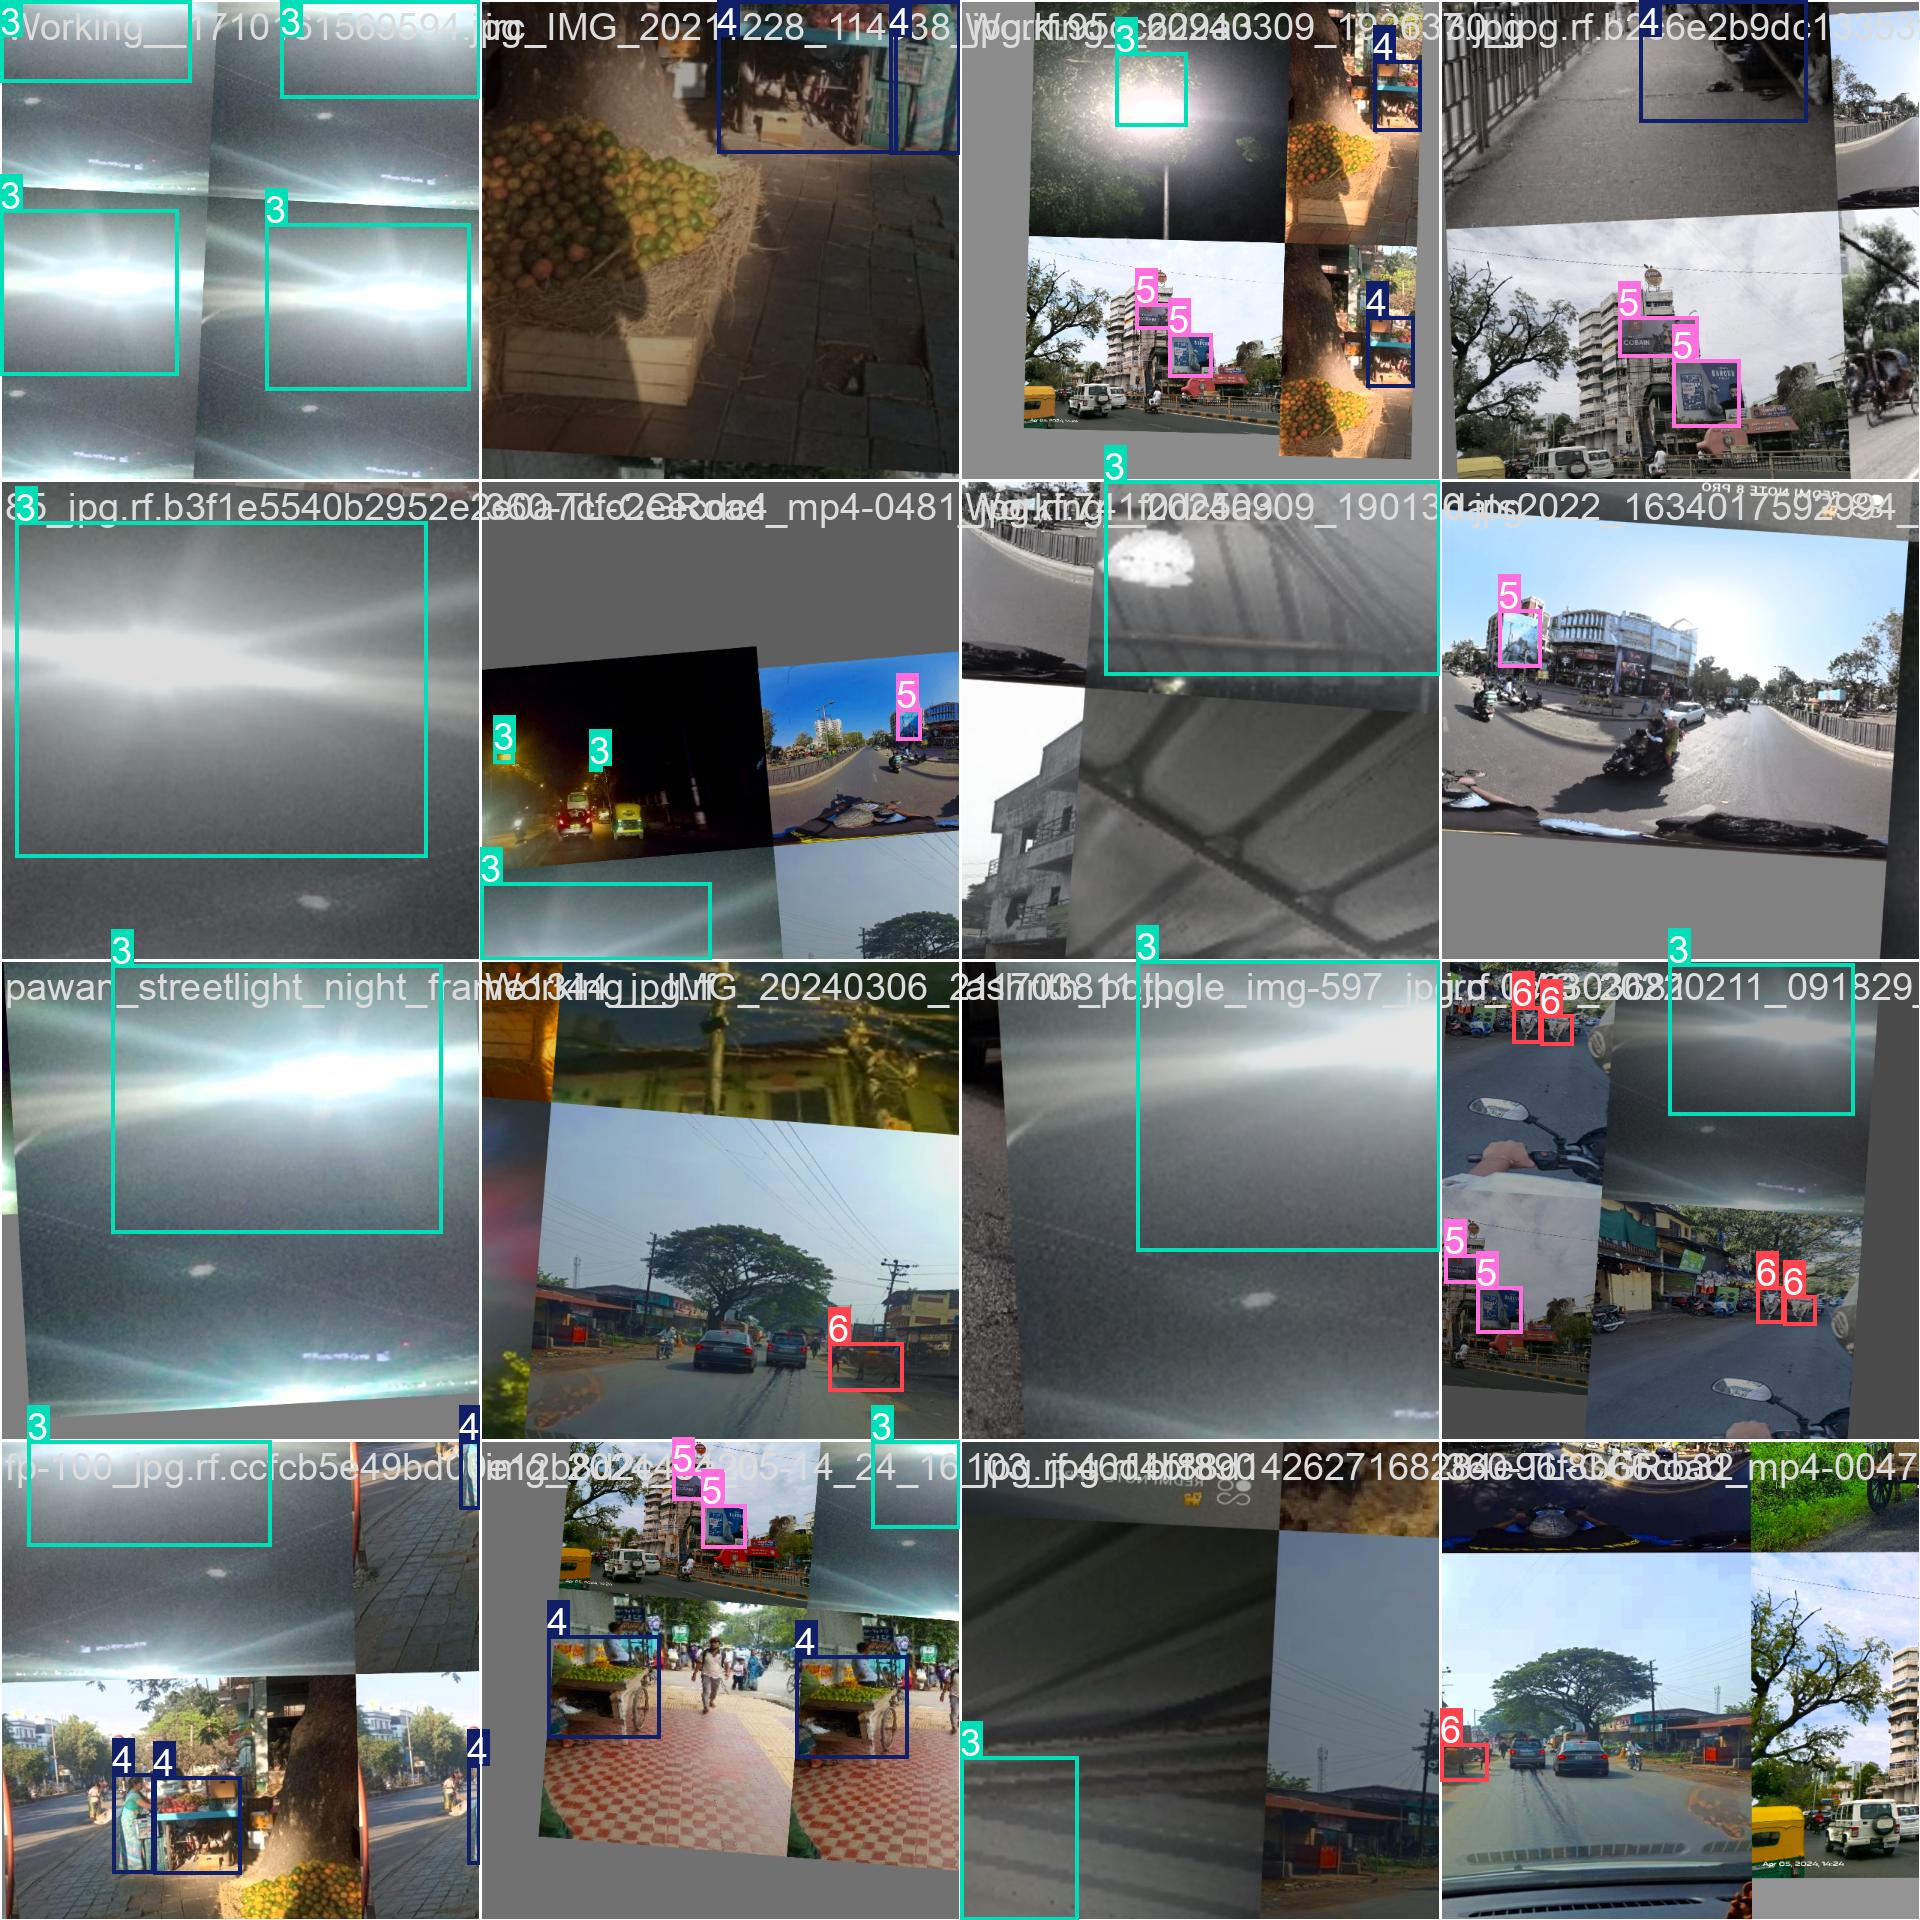
\includegraphics[width=0.72\textwidth]{images/oversampled_train_batch.jpg}
  \caption{A training mosaic batch from the oversampled run, showing the augmentation
  pipeline in effect (mosaic, copy-paste, color jitter) — this is what the model actually
  sees per step, including duplicated minority-class crops pasted onto other scenes.}
\end{figure}

% =====================================================================
\section{Extra Work: Data Extraction \& Class-Quality Improvement}
% =====================================================================
Alongside the two training runs above, ongoing work is targeted specifically at
improving the weakest classes and fixing label-quality defects, rather than just adding
more raw volume.

\subsection{Review \& Annotation Dashboard (\texttt{review\_annotate\_dashboard.py})}
A live, LAN-reachable Flask dashboard (port 5053) queues newly sourced candidate images
per class from \texttt{data/new\_review\_data/} — these arrive with auto-remapped boxes
from their source datasets, shown pre-drawn and editable rather than annotated from
scratch. It also surfaces the 17 legitimate empty-label \texttt{streetlight\_pole}
negatives already inside \texttt{data/re-training\_data}. A dedicated
\texttt{\_background\_negatives} queue was added to start building genuine
no-object-of-interest training samples, directly targeting the model's long-standing
lack of a background class (a confirmed source of confident false positives on
out-of-distribution input in earlier testing). Reviewer decisions persist in
\texttt{data/annotation\_review\_progress.json} so the queue only ever shows what is
still pending.

\subsection{Class Balancing (\texttt{balance\_train\_data.py})}
Round-robin duplicates minority-class train images/labels up to the current largest
class's count, writing to both the flat \texttt{data/re-training\_data} tree (what
\texttt{train.py} reads) and the per-class \texttt{data/classwise\_data} mirror so the
two stay in sync. Val/test are never touched, keeping evaluation on genuine, non-duplicated
data regardless of how training is balanced. This is what produced the
\texttt{civic\_services\_oversampled} run analyzed above.

\subsection{Billboard Annotation-Format Defect — Found and Partially Fixed}
While comparing the two runs, 21 \texttt{billboard\_hoarding} label files were found
mixing two incompatible annotation formats: plain YOLO boxes (\texttt{class cx cy w h},
5 fields) and segmentation polygons (\texttt{class x1 y1 x2 y2 ...}, an odd field count
$>5$). Ultralytics silently drops any file mixing both formats during train/val
(\texttt{"labels mix segment and detection rows"}), so these images were contributing
nothing. All 21 affected files traced back to a single source, \texttt{pawan\_billboard} —
the same source separately found to be $\sim$29\% non-Indian stock photography (Bangkok,
Buenos Aires, Rayong, Chonburi) by filename inspection, and which supplied
\emph{100\% of the val and test billboard\_hoarding images} before this fix, meaning the
class's reported AP50 (0.89--0.92 above) was being measured on an unrepresentative,
partly-foreign held-out set.

A purpose-built dashboard, \texttt{billboard\_format\_review.py} (port 5054), was written
to triage this: it classifies every \texttt{billboard\_hoarding} label file into
\emph{YOLO box (clean)}, \emph{segmentation only}, or \emph{mixed}, renders polygons and
their derived bounding boxes for visual comparison, and lets a reviewer convert, edit, or
reject each one. The dashboard \textbf{live-rescans} the dataset on a short TTL (rather
than a one-time snapshot at startup) and polls for changes every 4 seconds, so it reflects
edits made directly on disk — e.g.\ by an external cleanup script — without needing a
restart.

All 21 affected files were removed directly from \texttt{data/re-training\_data} and
\texttt{data/classwise\_data} (image + label pairs, both locations kept in sync).
\texttt{billboard\_hoarding} counts after cleanup:

\begin{table}[H]
\centering
\caption{billboard\_hoarding counts before/after removing the 21 format-defective files.}
\begin{tabular}{lccc}
\toprule
\textbf{Split} & \textbf{before} & \textbf{after} & \textbf{removed} \\
\midrule
train & 279 & 262 & 17 \\
val   & 10  & 6   & 4 \\
test  & 10  & 10  & 0 \\
\bottomrule
\end{tabular}
\end{table}

\noindent\textbf{Not yet done}: the val/test split is still not re-diversified across
sources (val is currently the remaining \texttt{pawan\_billboard} images only) — a proper
re-shuffle across all \texttt{billboard\_hoarding} sources is needed before this class's
metrics can be trusted, and a retrain is needed to reflect the cleaned label set.

% =====================================================================
\section{Summary \& Recommendations}
% =====================================================================
\begin{itemize}
  \item \textbf{No clean winner between the two runs} — oversampled trades mAP50/precision
    for recall and helps the two classes \texttt{copy\_paste} targets, but regresses the
    largest class (\texttt{streetlight\_pole}). Neither should be deployed as-is without
    addressing \texttt{garbage\_pile}'s weakness and the \texttt{billboard\_hoarding}
    split issue first.
  \item \textbf{Overfitting is present in both}, more so in oversampled due to image
    duplication; \texttt{best.pt} already mitigates this by selecting the best epoch, but
    tightening \texttt{patience} would save training time with no expected quality loss.
  \item \textbf{garbage\_pile needs investigation} — its AP50 collapsed relative to
    historical numbers on the older dataset; check the newly added
    \texttt{data/new\_review\_data/garbage\_pile} images for label-quality issues.
  \item \textbf{Billboard val/test split needs re-shuffling} across all sources, not just
    \texttt{pawan\_billboard}, before its metrics can be trusted; a retrain is needed after
    that to pick up the 21 removed files' absence and any re-split changes.
\end{itemize}

\end{document}
